% !TEX root = ../main.tex
\chapter{系统核心功能实现}

本章在前文系统设计的基础上，围绕 HearBridge 系统的核心功能实现过程展开说明。
与系统设计章节侧重架构划分、模块职责和数据关系不同，本章更关注各功能模块在工程代码中的落地方式，包括移动端页面状态组织、接口封装、实时识别通信、句子视频识别调用、服务端业务编排、后台管理端页面实现以及模型版本发布联动等内容。

根据当前项目实际结构，HearBridge 的系统实现主要由 HarmonyOS 移动端、Spring Boot 服务端、Vue 后台管理端和 Python 手势识别服务协同完成。
其中，移动端负责用户交互和结果展示，服务端负责业务数据管理和跨服务调用，后台管理端负责资源与模型维护，Python 识别服务负责实时识别、样本处理、模型训练与模型运行时管理。
考虑到手势识别模型结构、特征构造和实验结果具有较强算法属性，本文将其放在第六章集中说明；
本章只从系统功能接入和业务实现角度说明识别服务如何与主系统协作。

% !TEX root = ../../main.tex

\section{HarmonyOS 移动端核心模块实现}

HarmonyOS 移动端是普通用户使用系统的主要入口，主要实现登录认证、首页入口、手语资源浏览、手势训练、实时识别、句子视频识别和个人中心等功能。
移动端实现的重点是将后端资源数据、Python 实时识别能力和句子视频识别结果组织为用户可操作的页面流程，使用户能够顺利完成从资源选择到训练反馈的完整操作。

移动端核心页面效果如图~\ref{fig:chapter05-mobile-core-ui} 所示。

\begin{figure}[H]
  \centering

  \begin{subfigure}[t]{0.235\textwidth}
    \centering
    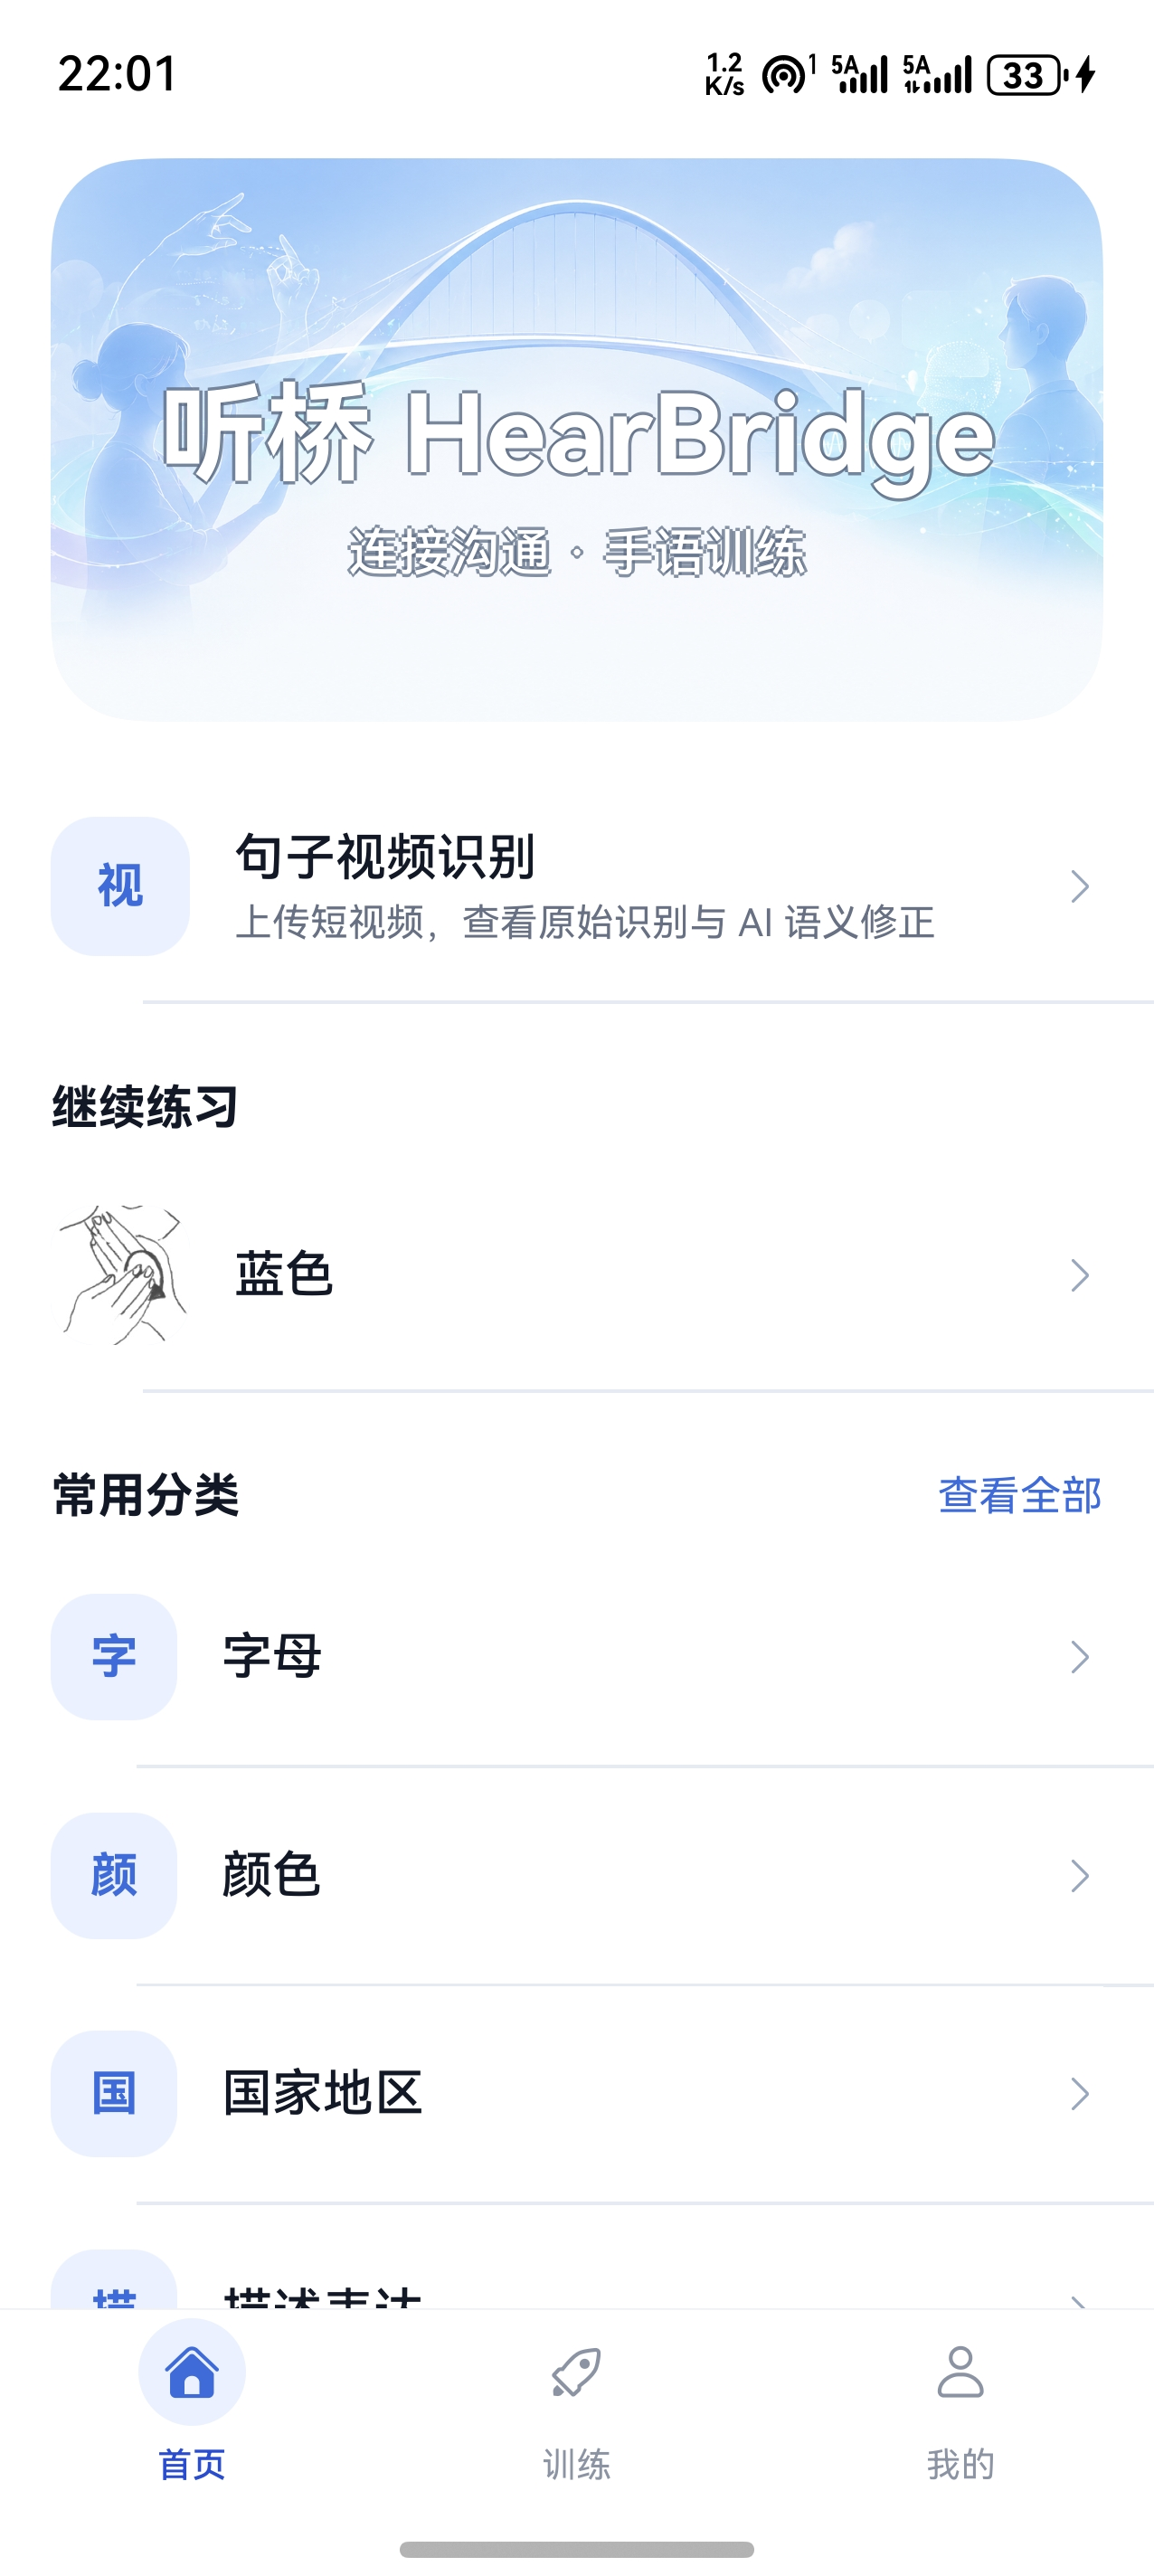
\includegraphics[width=\textwidth,height=0.32\textheight,keepaspectratio]{figures/chapter05/home-page.jpg}
    \caption{首页}
  \end{subfigure}
  \hfill
  \begin{subfigure}[t]{0.235\textwidth}
    \centering
    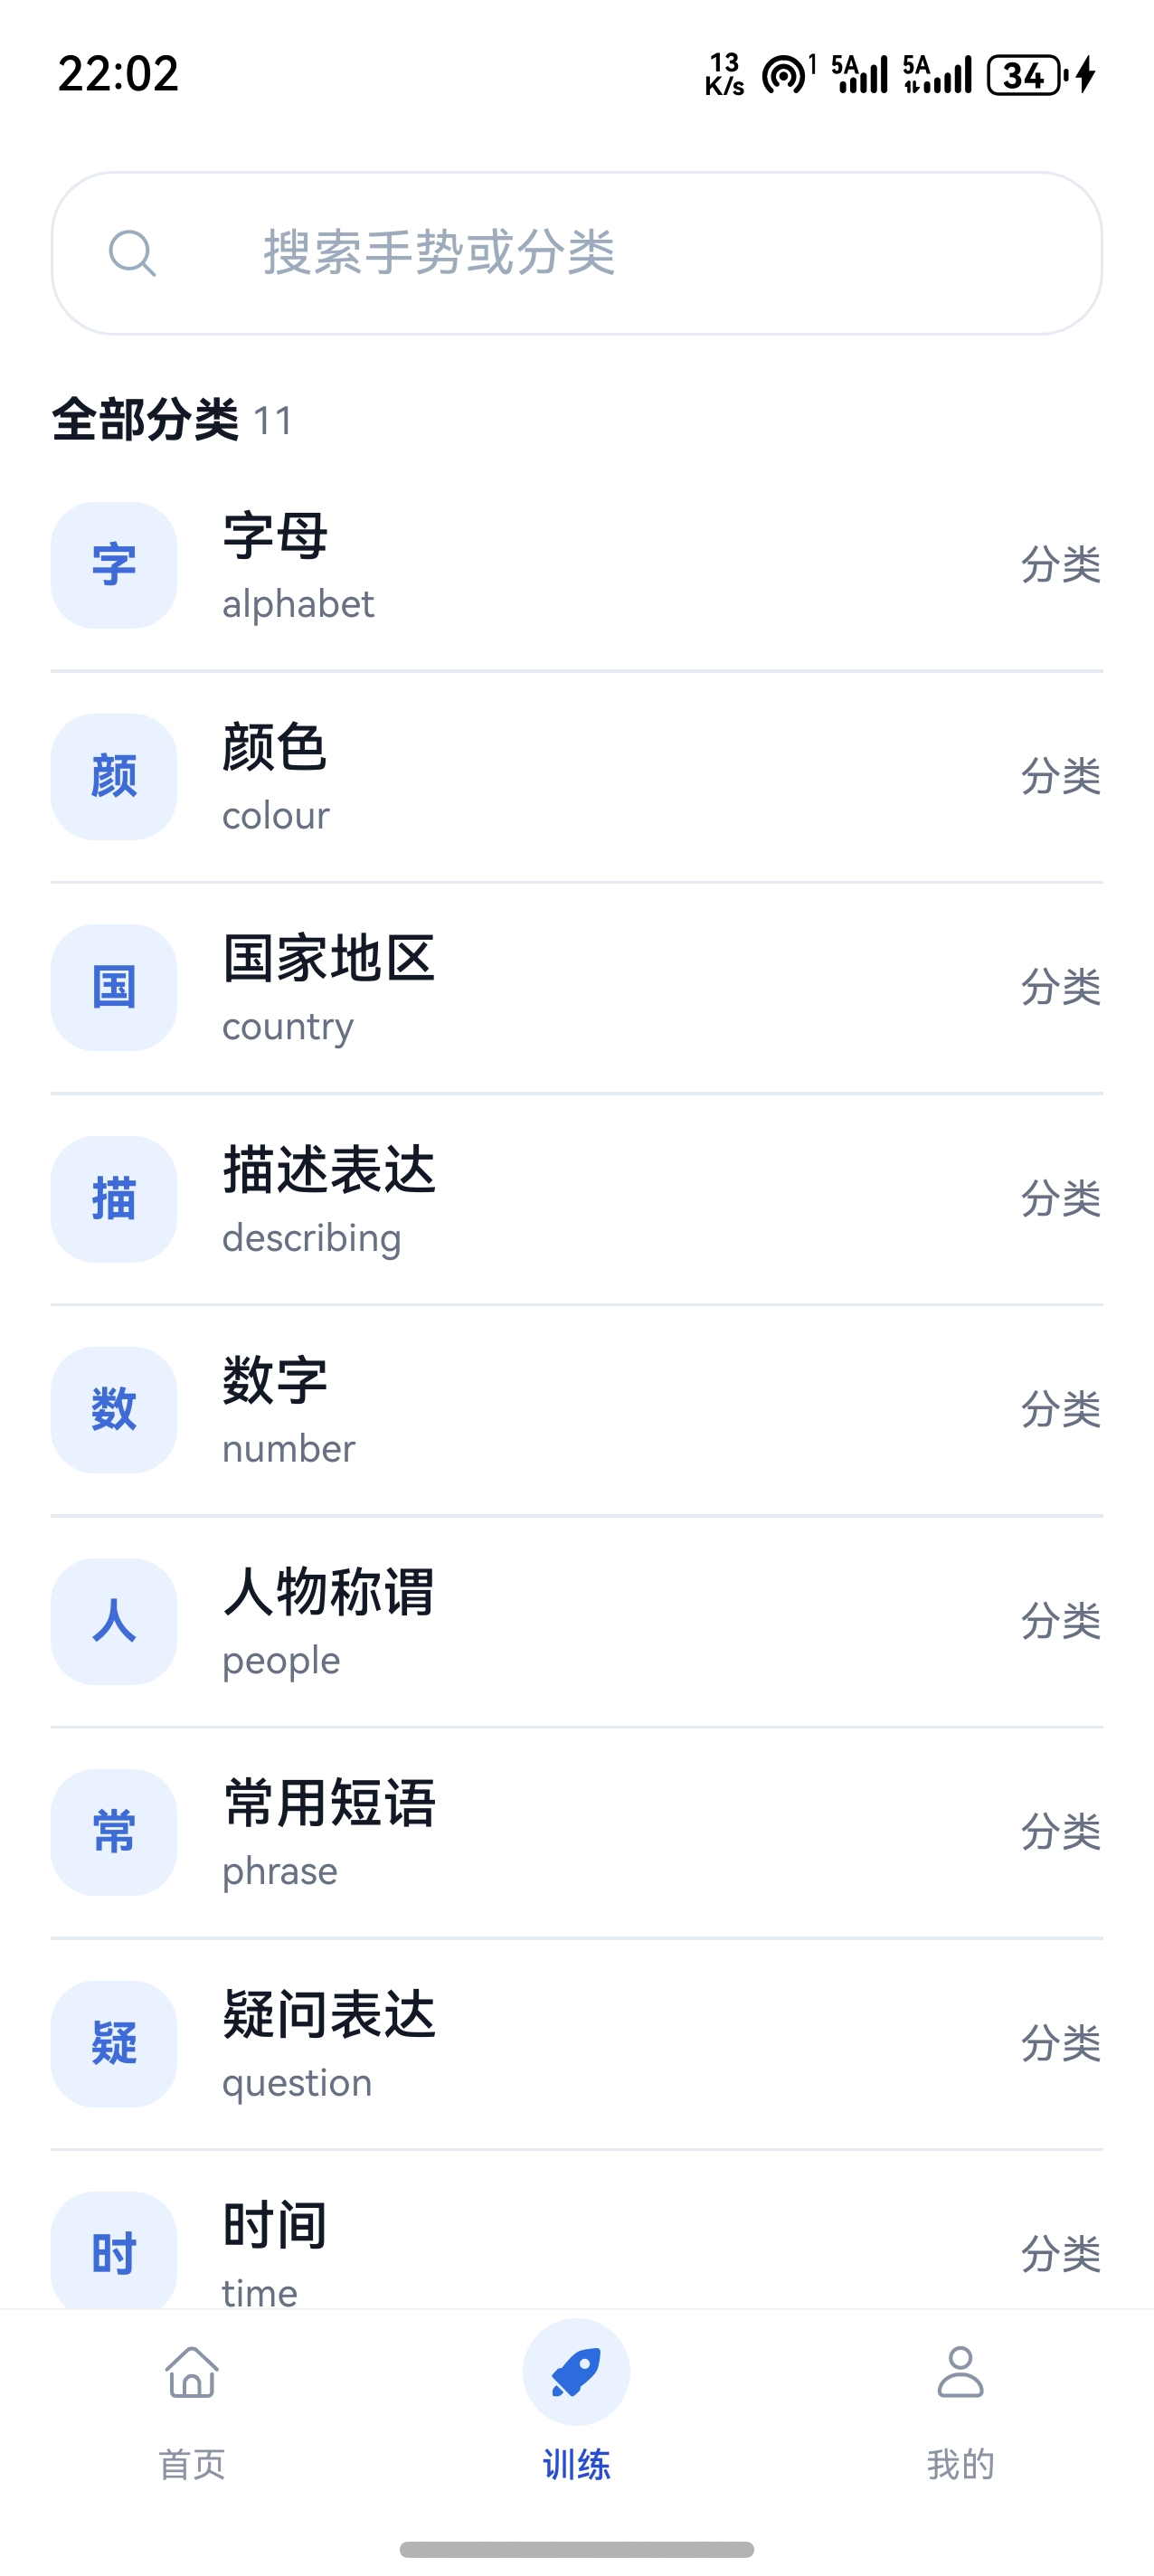
\includegraphics[width=\textwidth,height=0.32\textheight,keepaspectratio]{figures/chapter05/training-page.jpg}
    \caption{训练页}
  \end{subfigure}
  \hfill
  \begin{subfigure}[t]{0.235\textwidth}
    \centering
    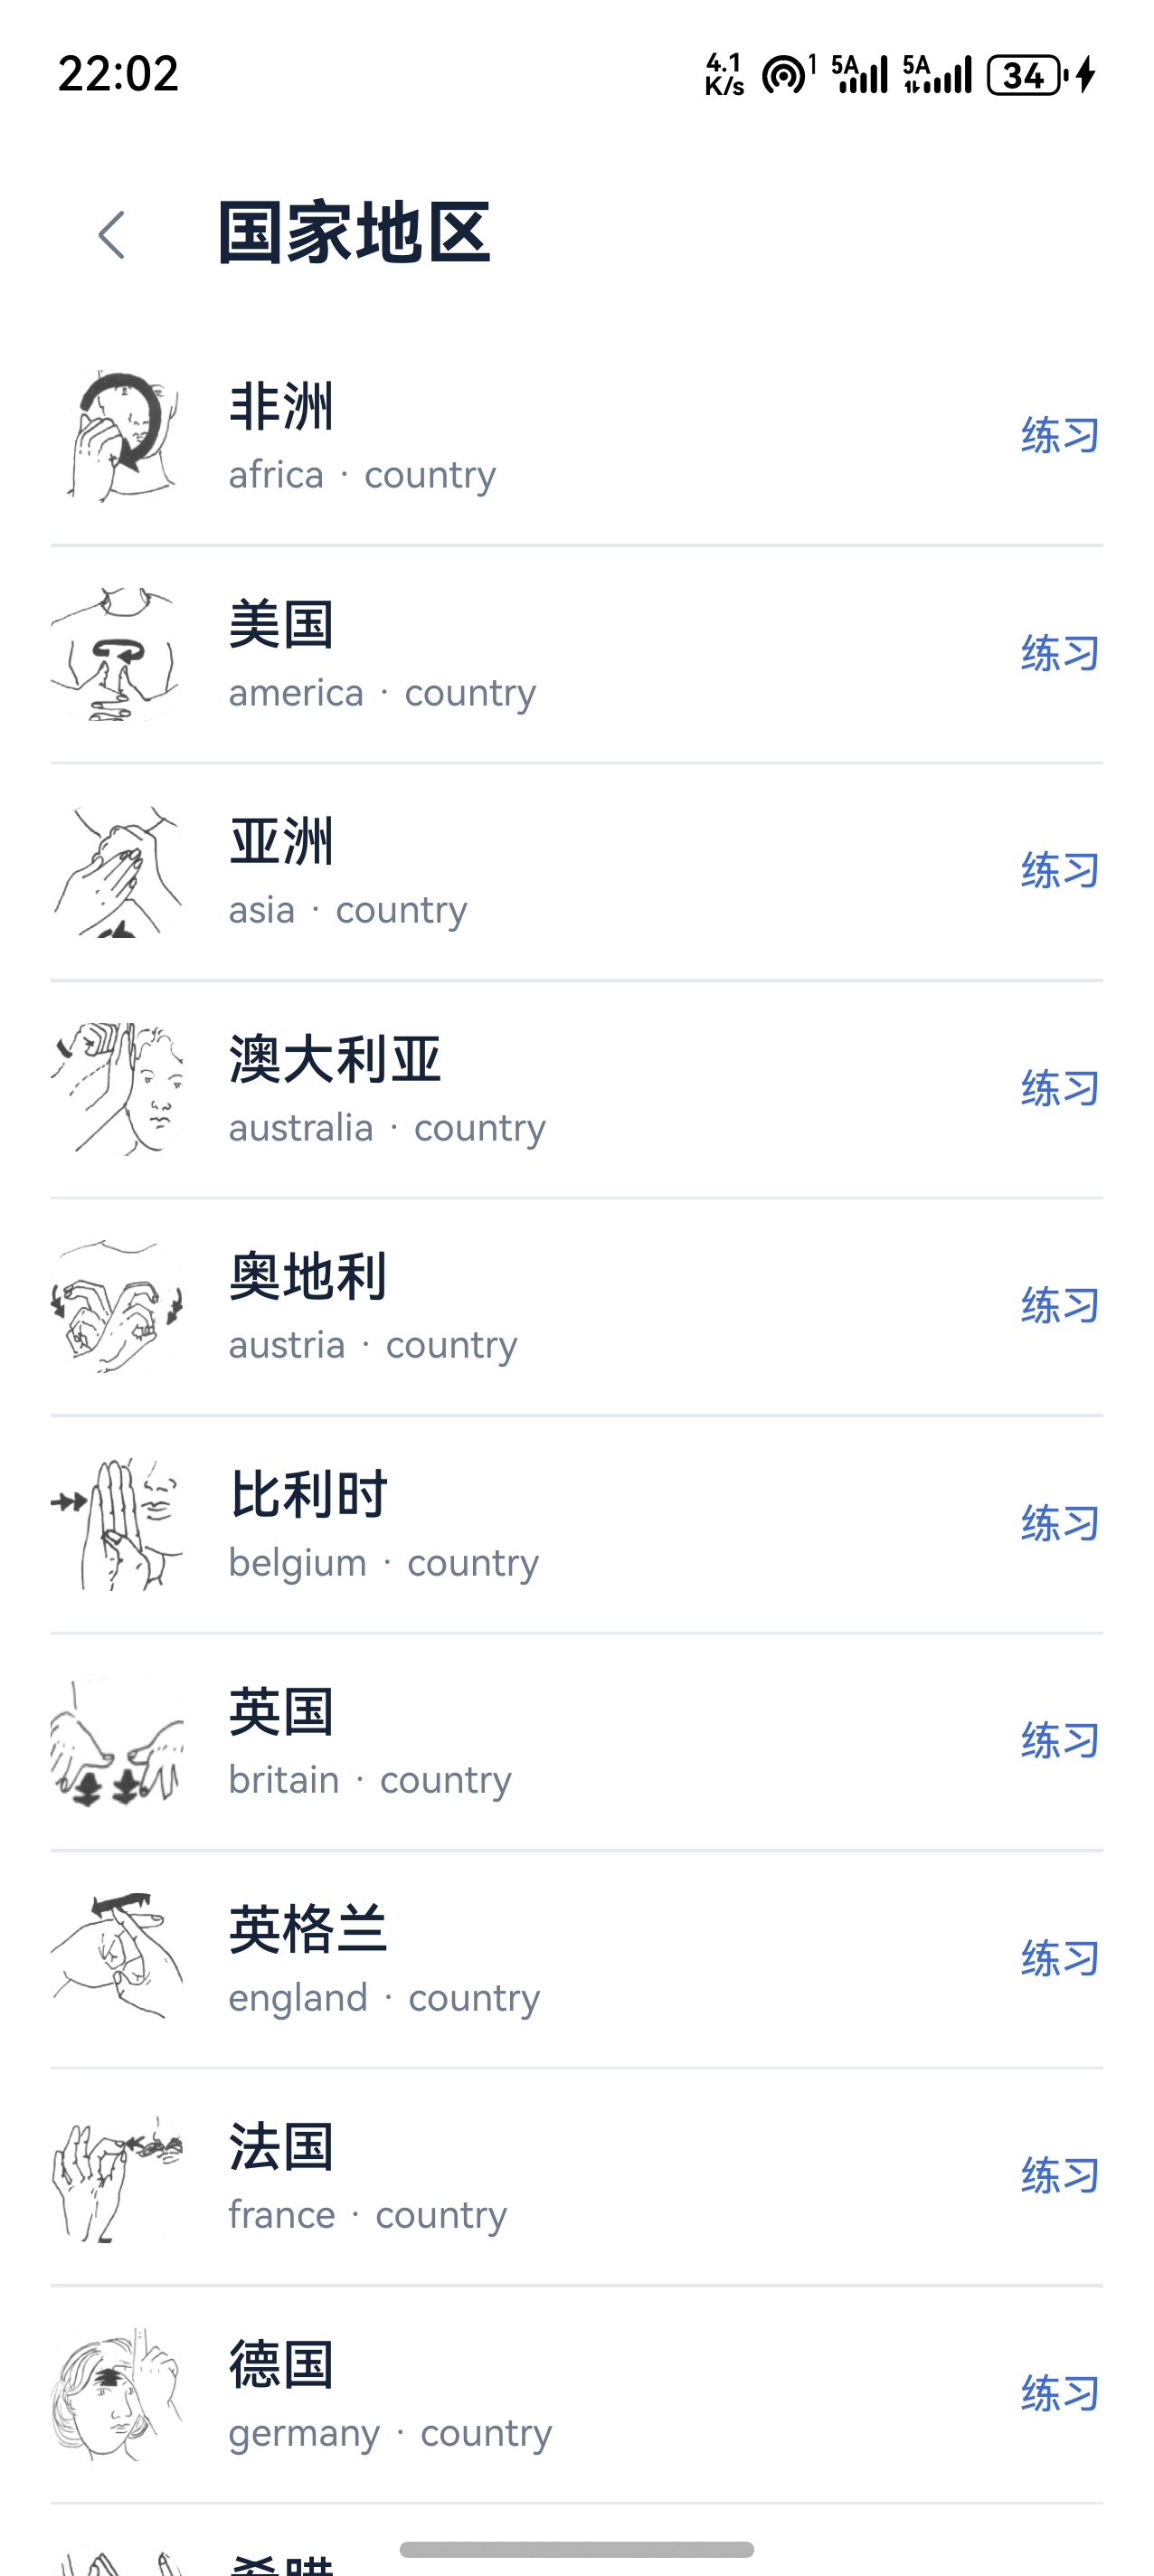
\includegraphics[width=\textwidth,height=0.32\textheight,keepaspectratio]{figures/chapter05/resource-list-page.jpg}
    \caption{资源列表页}
  \end{subfigure}
  \hfill
  \begin{subfigure}[t]{0.235\textwidth}
    \centering
    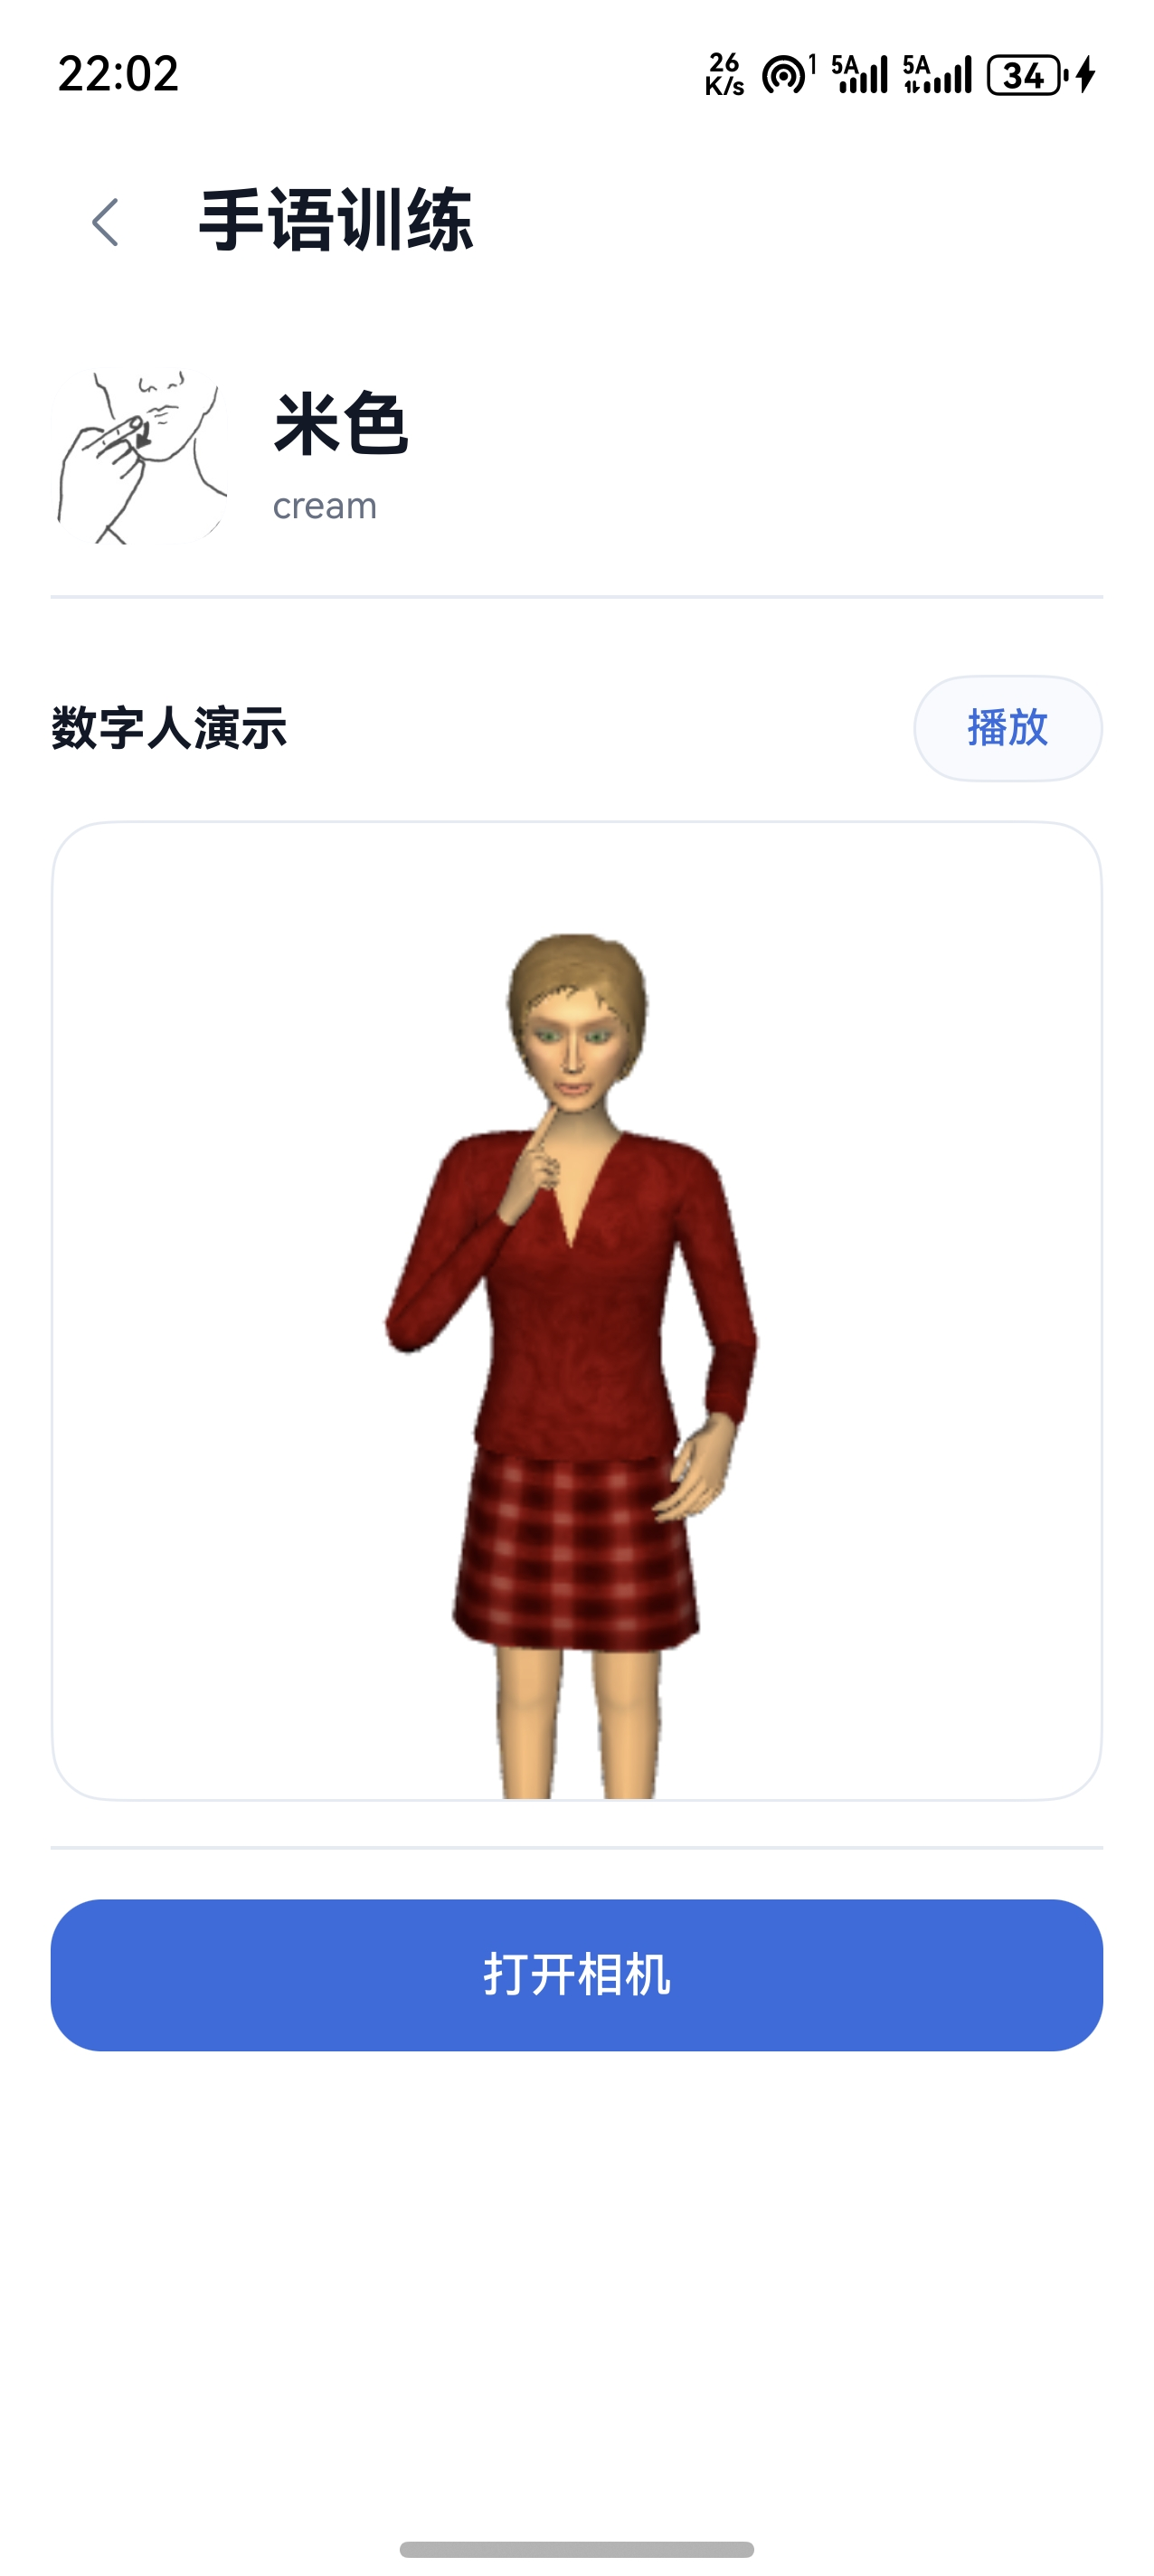
\includegraphics[width=\textwidth,height=0.32\textheight,keepaspectratio]{figures/chapter05/gesture-training-page.jpg}
    \caption{手势训练页}
  \end{subfigure}

  \caption{移动端核心页面效果图}
  \label{fig:chapter05-mobile-core-ui}
\end{figure}

移动端主要调用接口如表~\ref{tab:chapter05-mobile-interfaces} 所示。

\WhuInterfaceTable{移动端主要接口}{tab:chapter05-mobile-interfaces}{
登录认证 & POST & /app/auth/login & 普通用户登录并获取 token \\
用户信息 & GET & /app/user/profile & 获取当前登录用户信息 \\
手势分类 & GET & /app/sign/categories & 获取移动端可见手势分类 \\
手势资源 & GET & /app/sign/resources & 获取可训练手势资源列表 \\
最近练习 & GET & /app/recent-practice & 获取用户最近练习记录 \\
视频识别 & POST & /app/video-recognition & 上传句子视频并获取识别结果 \\
}

\subsection{应用启动、登录恢复与主界面组织实现}

应用启动后首先需要判断用户是否已经登录，并据此决定展示登录注册入口还是进入主界面。
当前移动端入口页面采用登录态驱动的页面切换方式，核心状态由全局登录状态控制。
页面出现时调用初始化逻辑，依次完成登录态恢复、最近练习记录恢复和手语分类加载。

在实现上，应用入口通过 aboutToAppear() 触发 initPage()，再由 restoreAuthState() 恢复本地登录态，由 restoreRecentPracticeFromBackend() 尝试恢复最近练习记录，最后调用 loadCategories() 通过 GestureApi 获取分类数据。
通过这种启动流程，应用能够在用户重新打开时自动恢复登录状态，并尽可能展示最近一次训练相关内容，减少用户重复操作。

主界面采用首页、训练、句子视频识别和个人中心等功能入口组织用户操作路径。
用户登录后，可以从首页查看手语资源和最近练习内容，也可以直接进入训练功能或句子视频识别功能。
个人中心则负责展示用户资料、修改密码和退出登录等操作。
通过这种入口组织方式，移动端将学习、训练、识别和个人管理功能聚合在统一应用内，减少用户在不同功能之间切换时的理解成本。

移动端页面状态主要围绕登录状态、分类列表、最近练习记录、识别结果和用户信息等数据展开。
页面本身不直接承担复杂业务处理，而是通过接口服务和状态管理对象获取数据、更新界面和响应用户操作。
该实现方式符合 HarmonyOS 声明式界面开发特点，也便于后续扩展新的训练入口或识别结果展示形式。

\subsection{手语资源浏览与训练入口实现}

手语资源浏览功能用于向用户展示可学习和训练的手语资源。
移动端在首页或资源页面加载分类数据后，根据分类进一步展示手语资源列表。
用户可以通过资源名称、分类入口或最近练习记录进入具体训练流程。
资源列表中的每一项通常包含资源名称、分类信息、封面或示范资源入口等内容，用于帮助用户快速判断该资源是否为当前需要练习的动作。

在资源浏览实现中，移动端主要通过后端接口获取手势分类和手势资源数据。
分类数据用于构建页面中的分类入口，资源数据则用于构建具体训练项。
由于资源内容由后台管理端维护，移动端不需要在本地写死训练动作，而是根据服务端返回的数据动态展示。
这样，当管理员在后台新增、修改或禁用手势资源后，移动端可以通过接口获取最新资源列表，从而提高系统内容维护的灵活性。

用户选择某个手语资源后，移动端进入训练准备或训练详情页面。
该页面需要展示动作名称、动作说明和标准动作示范入口，并为实时识别训练提供启动按钮。
若资源关联了数字人动作示范或视频资源，移动端可以在训练前展示对应动作，使用户先观察标准动作，再开始模仿训练。
该过程构成了移动端训练功能中的“标准动作展示”阶段。

训练入口的实现重点在于将资源数据、示范资源和识别服务入口连接起来。
用户点击训练按钮后，移动端需要根据当前资源信息构建识别上下文，包括当前训练动作、资源标识和后续结果展示所需的数据。
通过这种方式，移动端能够将资源浏览过程自然过渡到实时训练过程，使用户操作路径从“选择资源”进入“动作练习”。

\subsection{实时手势训练交互实现}

实时手势训练是移动端的核心功能之一。
用户进入训练页面后，应用调用相机采集图像帧，并通过 WebSocket 与 Python 手势识别服务建立实时通信。
移动端持续发送相机图像帧，识别服务返回当前窗口的预测标签、置信度、模型版本等结果，移动端再将识别结果展示给用户。

在实现过程中，移动端需要处理相机权限、相机预览、图像帧获取、WebSocket 连接、识别结果解析和页面状态更新等多个环节。
相机预览用于给用户提供动作调整依据，图像帧发送用于给 Python 识别服务提供输入，识别结果展示则用于形成训练反馈。
为了降低用户等待感，移动端在识别过程中需要及时展示连接状态、识别状态和结果状态，使用户能够判断当前系统是否正在工作。

实时识别结果通常包含预测动作、置信度和模型版本等信息。
移动端接收到结果后，根据当前训练资源和识别结果进行展示。
如果识别结果与当前训练动作一致，可以向用户展示较积极的反馈；
如果识别结果不一致，则可以提示用户调整动作。
当前实现重点并不在移动端完成复杂评分，而是将 Python 识别服务返回的结果组织为用户可理解的训练反馈。

为了保证训练体验，移动端还需要处理识别连接断开、相机帧为空、识别服务异常等情况。
当 WebSocket 连接失败或识别服务不可用时，页面应给出明确提示，而不是让用户停留在无反馈状态。
通过这些状态处理，移动端实时训练功能能够在较复杂的设备和网络环境下保持可用性。

\subsection{句子视频识别页面实现}

除实时单词训练外，移动端还支持句子视频识别功能。
用户可以在移动端选择本地手语句子视频，并提交给服务端进行识别。
服务端接收视频文件后调用 Python 手势识别服务进行视频分析，再结合语义修正服务组织最终结果。
移动端负责展示识别过程状态、原始识别结果、中文映射结果和语义修正结果。

句子视频识别页面效果如图~\ref{fig:chapter05-video-recognition-page} 所示。

\WhuImageFigure[0.42\textwidth][0.68\textheight]{figures/chapter05/video-recognition-page.jpg}{句子视频识别页面效果图}{fig:chapter05-video-recognition-page}

句子视频识别功能的实现过程与实时识别不同。
实时识别强调相机帧的连续传输和即时反馈，而句子视频识别强调视频文件上传、服务端异步处理和结果展示。
移动端在用户选择视频后，需要完成文件选择、上传请求构建、等待识别结果和展示识别结果等步骤。
由于视频识别耗时可能比实时单帧识别更长，页面需要展示加载状态，避免用户误以为操作失败。

识别结果展示时，移动端通常需要区分原始结果和修正结果。
原始结果体现模型识别出的词级序列或候选结果，中文映射结果用于将标签转化为用户可理解的中文词语，语义修正结果则用于展示经过语言组织后的句子表达。
通过分层展示这些结果，用户既可以看到模型的基础识别输出，也可以看到更自然的句子级结果。

该功能体现了移动端与服务端、Python 识别服务和语义修正服务之间的协作关系。
移动端并不直接处理视频识别算法，而是负责将用户输入的视频提交到服务端，并将服务端返回的多层结果转化为清晰的页面展示。
这样可以保持移动端逻辑相对轻量，同时让识别算法和语义处理能力在服务端和识别服务中统一维护。

% !TEX root = ../../main.tex

\section{Spring Boot 服务端核心模块实现}

Spring Boot 服务端是系统业务中心，主要负责用户认证、资源管理、文件管理、句子视频识别编排、语义修正调用、模型版本管理和后台管理端接口支持。
与移动端和管理端相比，服务端的重点在于统一数据口径、完成权限校验、封装跨服务调用并维护业务状态。

服务端核心业务接口如表~\ref{tab:chapter05-backend-interfaces} 所示。

\WhuInterfaceTable{服务端核心业务接口}{tab:chapter05-backend-interfaces}{
认证管理 & POST & /app/auth/login & 普通用户登录认证 \\
管理员认证 & POST & /admin/auth/login & 后台管理员登录认证 \\
分类管理 & GET/POST & /admin/sign/categories & 手势分类查询与维护 \\
资源管理 & GET/POST & /admin/sign/resources & 手势资源查询与维护 \\
样本管理 & GET/POST & /admin/sign/samples & 手势样本查询与维护 \\
视频识别 & POST & /app/video-recognition & 上传句子视频并组织识别结果 \\
语义修正 & POST & /app/semantic-correction & 根据识别词序列生成语义修正结果 \\
文件上传 & POST & /file/upload & 上传封面、视频、样本或模型文件 \\
模型版本 & GET/POST & /admin/model-versions & 模型版本登记与查询 \\
模型发布 & POST & /admin/model-versions/publish & 发布模型并联动识别服务加载 \\
}

\subsection{服务端分层结构实现}

服务端采用控制器层、服务层、持久层和外部服务客户端相结合的结构。
控制器层负责接收移动端和管理端 HTTP 请求，服务层负责业务规则处理和跨服务编排，持久层基于 MyBatis 完成数据库访问，外部服务客户端负责调用 Python 手势识别服务和 DeepSeek 服务。

当前服务端控制器按业务模块划分，主要包括 AppAuthController、AppUserController、AppRecentPracticeController、SignCategoryController、SignResourceController、SignSampleController、SignModelVersionController、SignVideoRecognitionController、SignSemanticCorrectionController、FileUploadController 等。
该划分方式与系统功能模块保持一致，使移动端、后台管理端和识别相关接口具有较清晰的入口。

服务端接口返回结构尽量保持统一，前端在调用时只需要关注业务数据和错误提示。
对于参数错误、登录状态失效、数据库异常、对象存储异常和识别服务异常，服务端通过统一异常处理机制转换为前端可理解的响应信息，避免直接暴露底层异常。
通过这种分层方式，服务端能够在保持接口结构清晰的同时，降低业务逻辑、数据库访问和外部服务调用之间的耦合。

\subsection{用户认证与登录态维护实现}

服务端同时支持普通用户和管理员两类认证场景。
普通用户认证面向 HarmonyOS 移动端，管理员认证面向 Vue 后台管理端。
两类登录流程在业务角色上相互区分，但基本思路一致：登录成功后生成 token，并将 token 与用户身份信息写入 Redis；
后续请求携带 token 时，服务端根据 Redis 中的登录态判断请求是否有效。

采用 Redis 保存登录态的原因在于，登录状态属于高频读取、短时效和可过期数据，不适合每次请求都访问 MySQL 进行校验。
服务端在用户退出登录或 token 过期后移除对应登录态，使客户端必须重新登录。
通过这种方式，系统既保证了接口访问控制，也降低了数据库认证压力。

在移动端场景中，用户登录成功后，移动端保存 token 和必要的用户信息，并在后续请求中携带 token。
服务端根据 token 查询 Redis 中的用户登录态，并将用户身份传递给后续业务逻辑。
对于后台管理端，管理员登录后同样获得 token，但服务端在处理后台接口时会区分管理员身份和权限场景，避免普通用户访问管理接口。

退出登录时，客户端主动调用退出接口，服务端删除 Redis 中对应登录态。
若 token 已经过期或不存在，服务端会向客户端返回登录失效信息，前端再跳转到登录页面或要求用户重新登录。
该流程使普通用户端和后台管理端都能够形成较完整的认证闭环。

\subsection{手语分类与手语资源服务实现}

手语分类和手语资源服务为移动端训练内容展示提供数据支撑，也为后台管理端资源维护提供接口。
分类服务主要负责分类列表查询、新增、修改、删除和状态控制；
资源服务主要负责手语资源的分页查询、详情查询、新增、修改、删除、启用禁用和资源文件关联等操作。

对于移动端，服务端主要提供已启用分类和已启用资源的查询接口。
移动端通过这些接口构建首页分类入口、资源列表和训练详情页面。
由于移动端面向普通用户，接口返回内容需要避免暴露过多后台维护字段，而是重点返回资源名称、分类信息、封面地址、示范资源地址和可训练状态等展示所需信息。

对于后台管理端，服务端提供更完整的分类和资源维护接口。
管理员可以在后台新增或修改分类，维护资源编码、资源名称、所属分类、封面资源、动作示范资源和启用状态等信息。
服务端在处理这些操作时需要完成参数校验、资源唯一性检查和数据库更新，保证移动端展示的数据具有一致性。

手语资源服务还承担连接训练流程和识别服务的作用。
资源编码或资源标签需要与 Python 识别服务中的标签体系保持对应关系，使移动端选择的训练资源能够与识别模型输出结果进行匹配。
因此，服务端在资源维护过程中不仅保存展示字段，也需要维护资源编码等与识别链路相关的关键字段。

\subsection{句子视频识别服务实现}

句子视频识别服务用于支持移动端上传手语句子视频，并获得词级识别结果、中文映射结果和后续语义修正结果。
该功能不由移动端直接调用 Python 识别服务完成，而是通过 Spring Boot 服务端进行统一编排。
这样可以避免移动端直接感知多个后端服务的调用细节，也便于服务端统一处理文件保存、接口调用、结果组织和异常提示。

用户在移动端选择本地手语视频后，移动端将视频文件上传到 Spring Boot 服务端。
服务端接收视频后，可以先将视频保存到对象存储或临时目录，再调用 Python 手势识别服务进行视频识别。
Python 服务读取视频帧，对视频中的动作片段进行关键点提取、特征构造和模型预测，生成词级识别结果。

与实时识别不同，句子视频识别需要从完整视频中提取动作序列，并尽可能生成连续词语结果。
Python 服务可以根据视频帧序列逐段识别手势动作，并输出原始标签序列或候选词序列。
由于模型识别结果可能存在重复、遗漏或顺序不够自然的问题，服务端还需要对识别结果进行初步整理。

Spring Boot 服务端在收到 Python 服务返回的结果后，负责将标签结果映射为中文词语，并组织原始识别结果、中文映射结果和待修正文本。
这样可以让系统保留模型原始输出，同时也为后续语义修正提供输入。
移动端最终展示时，可以将这些结果分层呈现给用户。

\subsection{DeepSeek 语义修正服务实现}

DeepSeek 语义修正服务用于将词级识别结果整理为更自然的中文表达。
由于当前系统定位为有限词表和受控场景下的手语辅助识别，模型输出往往是若干词语或短语序列，而不是完全符合汉语语序的自然句。
服务端通过调用 DeepSeek 语义修正服务，对识别结果进行语义组织和表达优化。

服务端在调用语义修正服务时，需要构造清晰的输入文本。
该输入通常包括识别出的中文词序列、任务说明和输出约束。
为了避免语义修正过度发挥，服务端应尽量要求模型基于已有识别结果进行整理，不随意添加识别结果中不存在的核心信息。
这样可以在提升可读性的同时，降低语义修正引入错误内容的风险。

语义修正服务返回结果后，Spring Boot 服务端将其与原始识别结果一起封装返回移动端。
移动端展示时，可以同时显示原始词序列和修正后的句子，使用户能够理解系统识别过程，也可以对比修正前后的表达差异。
该设计有助于提高结果透明度，避免用户只看到一个不可解释的最终句子。

需要注意的是，DeepSeek 在系统中只承担语义后处理职责，不直接参与视频视觉识别，也不替代手势识别模型。
视觉识别结果仍由 Python 手势识别服务生成，DeepSeek 只在识别候选结果的基础上完成语言表达整理。
通过这种分层处理方式，系统能够在保留识别链路可解释性的同时，提高句子结果的可读性。

\subsection{文件上传与资源访问实现}

系统中的头像、封面、动作示范资源、样本文件、视频文件和模型文件等都属于非结构化资源，不适合直接写入数据库。
服务端通过文件上传接口对接 MinIO 对象存储，将文件保存到对象存储中，并在数据库中记录文件访问地址和业务关联关系。
这样既可以避免数据库存储大文件，也便于后续扩展资源访问和文件管理能力。

文件上传模块通常由 FileUploadController 接收前端上传请求，再由文件服务完成文件名生成、存储路径组织、MinIO 上传和访问地址返回。
对于普通图片和视频资源，服务端返回的地址可以直接被移动端或后台管理端使用；
对于模型文件和样本文件，则需要与样本管理或模型版本管理模块建立业务关联。

在手势资源管理场景中，管理员可以上传资源封面、动作示范视频或数字人资源地址，服务端保存文件访问路径后，移动端即可通过资源接口获取并展示对应内容。
在句子视频识别场景中，移动端上传的视频文件可以由服务端临时保存或转发给 Python 识别服务处理。
对于训练样本和模型文件，服务端需要维护其业务归属和版本关系，避免资源文件与数据库记录脱节。

通过文件上传和资源访问模块，系统将结构化业务数据与非结构化文件资源分离存储。
MySQL 保存资源元数据、业务状态和关联关系，MinIO 保存具体文件内容，服务端则负责在二者之间建立映射。
这种设计有利于提升系统资源管理能力，也为后续更换对象存储或扩展文件类型提供了空间。

\subsection{关键接口调用说明}

HearBridge 系统的核心功能依赖多端之间的接口调用。
移动端主要调用普通用户认证、手势分类、手势资源、最近练习和视频识别等接口；
后台管理端主要调用管理员认证、分类管理、资源管理、样本管理、训练管理和模型版本管理等接口；
Spring Boot 服务端在部分业务中还需要调用 Python 手势识别服务和 DeepSeek 语义修正服务。

在实时手势训练场景中，移动端主要通过 WebSocket 与 Python 手势识别服务通信，持续发送图像帧并接收识别结果。
该链路强调连续帧传输和即时反馈，因此不适合通过普通 HTTP 接口反复请求完成。
在句子视频识别场景中，移动端通过 HTTP 上传视频文件，由 Spring Boot 服务端统一编排文件处理、Python 服务调用和语义修正调用。

在后台模型维护场景中，管理员通过后台管理端发起样本查询、模型训练和模型发布等请求。
Spring Boot 服务端负责将这些请求转化为业务操作，并在需要时调用 Python 识别服务完成特征转换、模型训练或模型重载。
模型发布成功后，移动端实时识别和视频识别功能才能使用当前发布模型。

接口调用过程中需要保持统一的数据格式和错误语义。
普通业务接口应返回统一响应结构，识别服务调用失败、文件上传失败、模型加载失败等异常需要被转换为前端可理解的提示信息。
通过统一接口封装和异常处理，系统能够降低多端联调复杂度，提高整体功能稳定性。

% !TEX root = ../../main.tex

\section{Vue 后台管理端核心模块实现}

Vue 后台管理端主要面向系统管理员，承担手势资源、样本数据、训练任务和模型版本等维护工作。
与移动端面向普通用户的训练识别流程不同，后台管理端更关注系统资源的可维护性和模型闭环的可管理性。
当前后台管理端基于 Vue 和 Element Plus 实现，通过统一请求封装访问 Spring Boot 服务端接口，并结合路由守卫和 token 机制完成后台访问控制。

后台管理端核心页面组织如图~\ref{fig:chapter05-admin-management-pages} 所示。

\begin{figure}[H]
  \centering
  \begin{subfigure}[t]{0.47\textwidth}
    \centering
    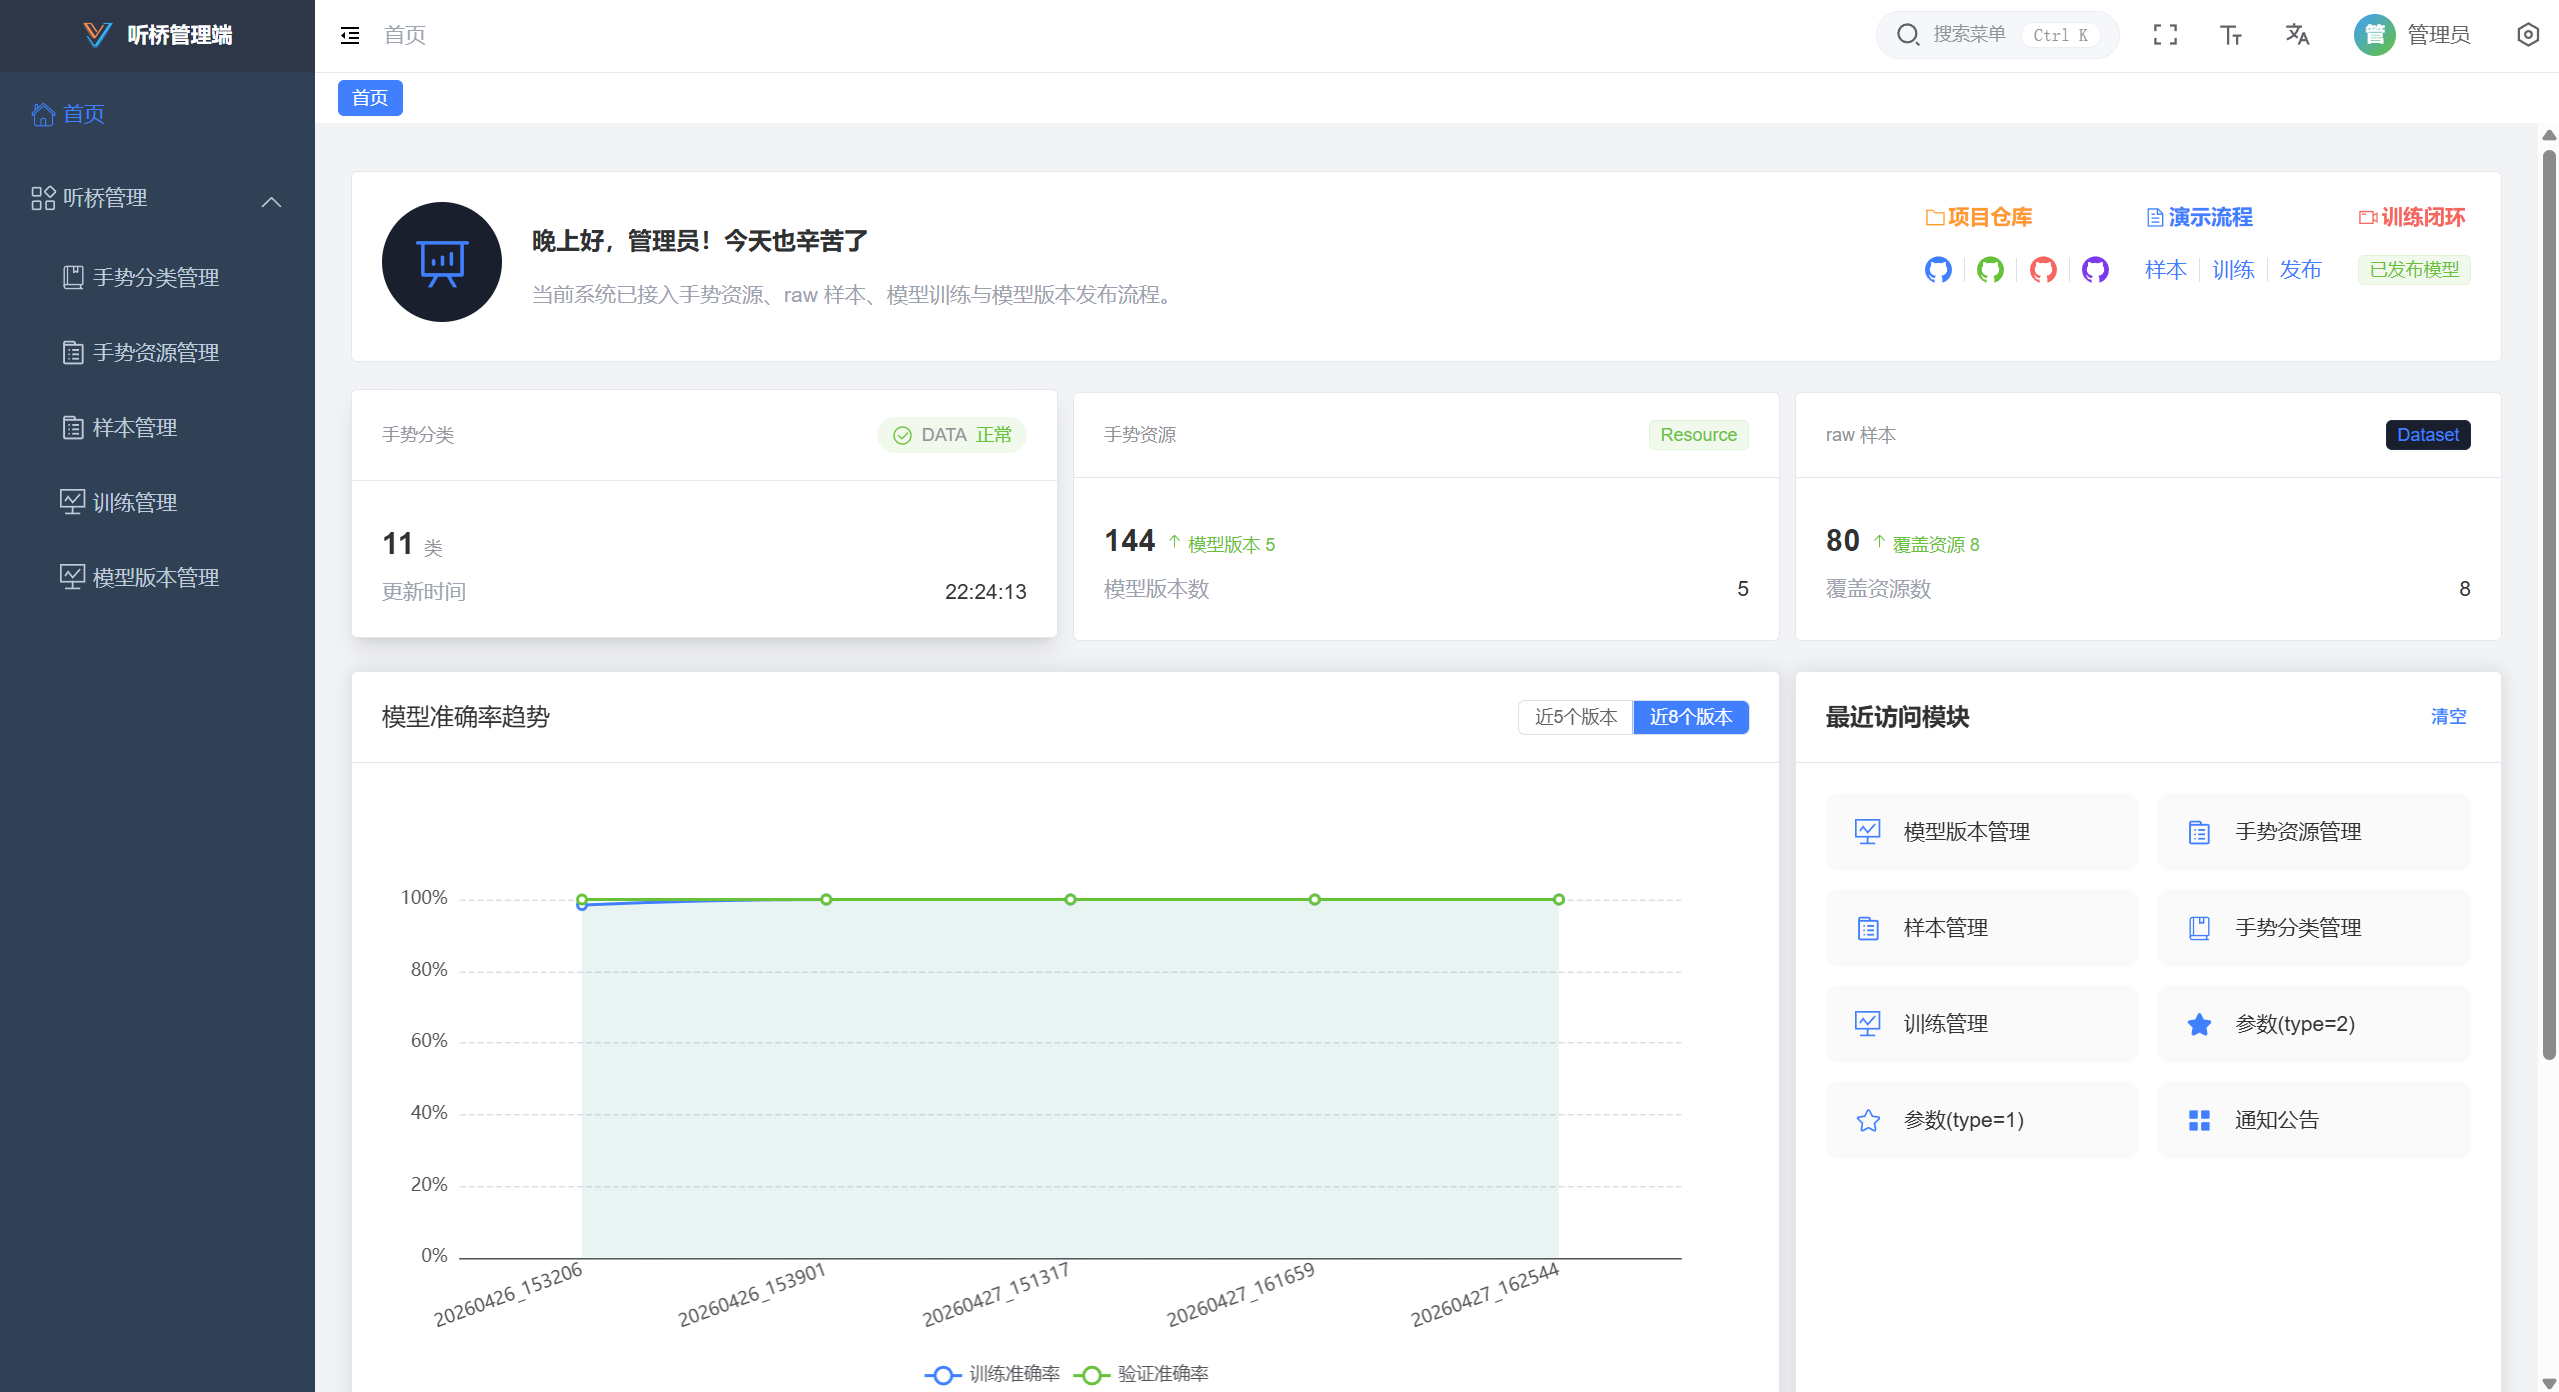
\includegraphics[width=\textwidth,height=0.23\textheight,keepaspectratio]{figures/chapter05/admin-system-overview.png}
    \caption{系统概览}
  \end{subfigure}
  \hfill
  \begin{subfigure}[t]{0.47\textwidth}
    \centering
    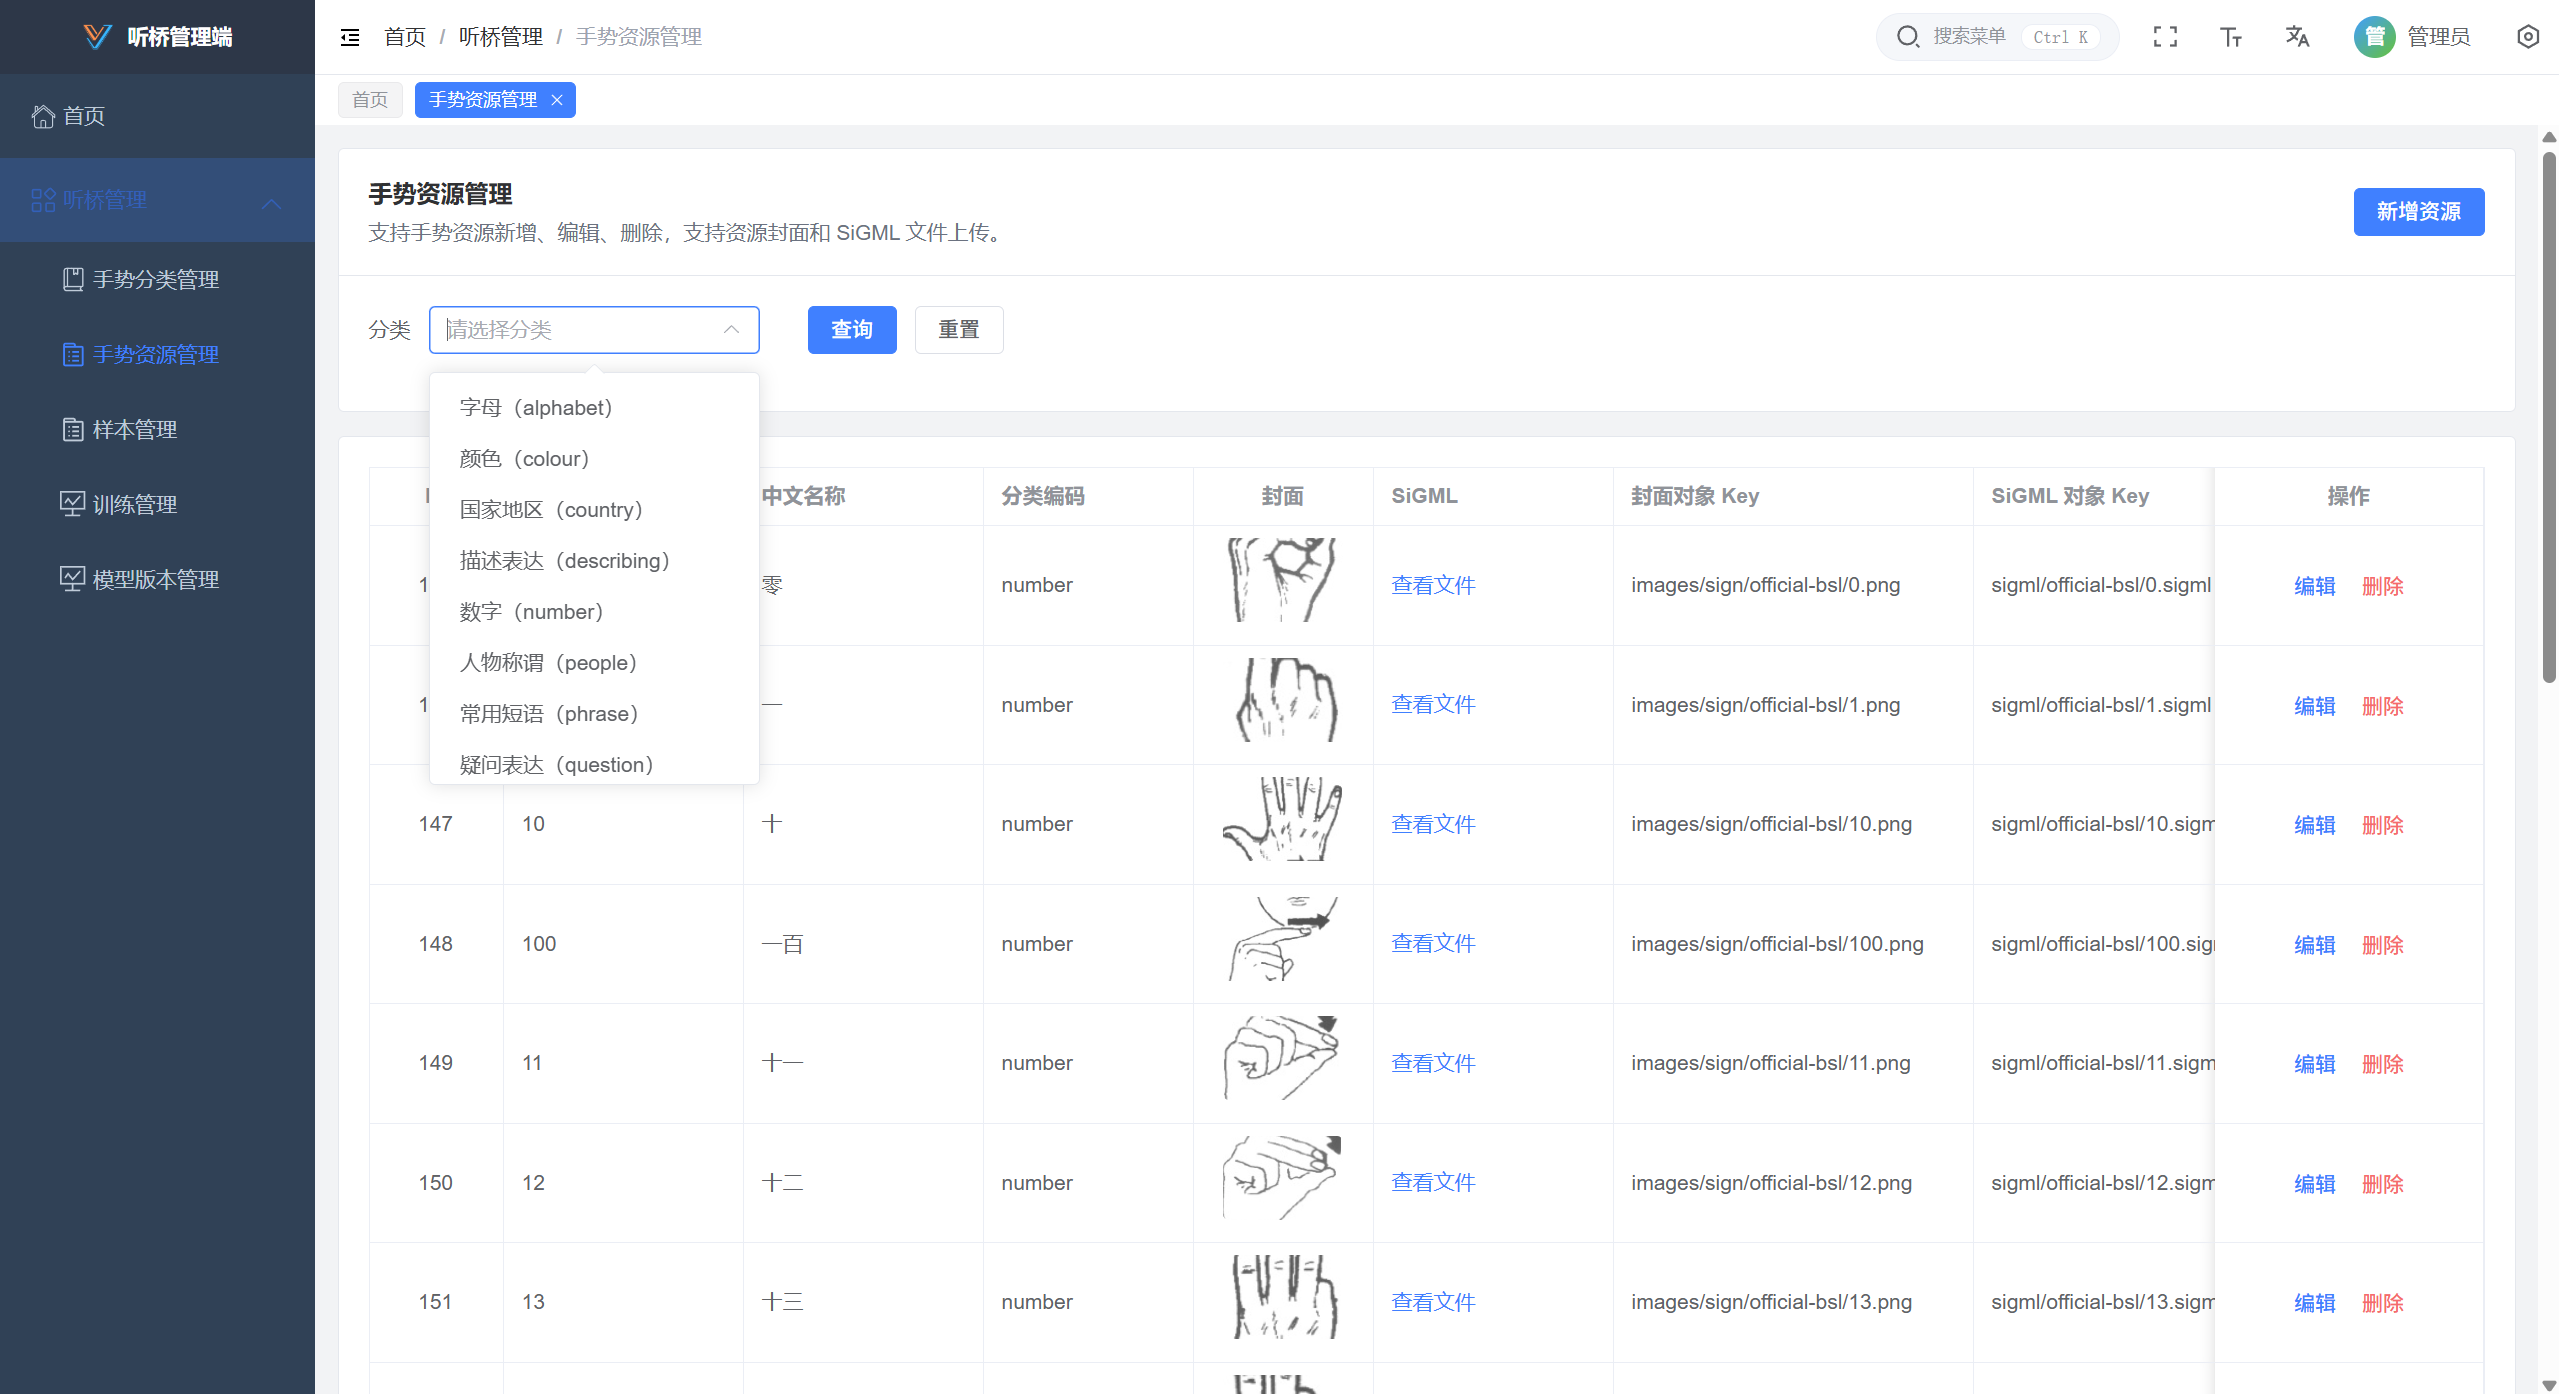
\includegraphics[width=\textwidth,height=0.23\textheight,keepaspectratio]{figures/chapter05/gesture-resource-management.png}
    \caption{手势资源管理}
  \end{subfigure}

  \vspace{6pt}

  \begin{subfigure}[t]{0.47\textwidth}
    \centering
    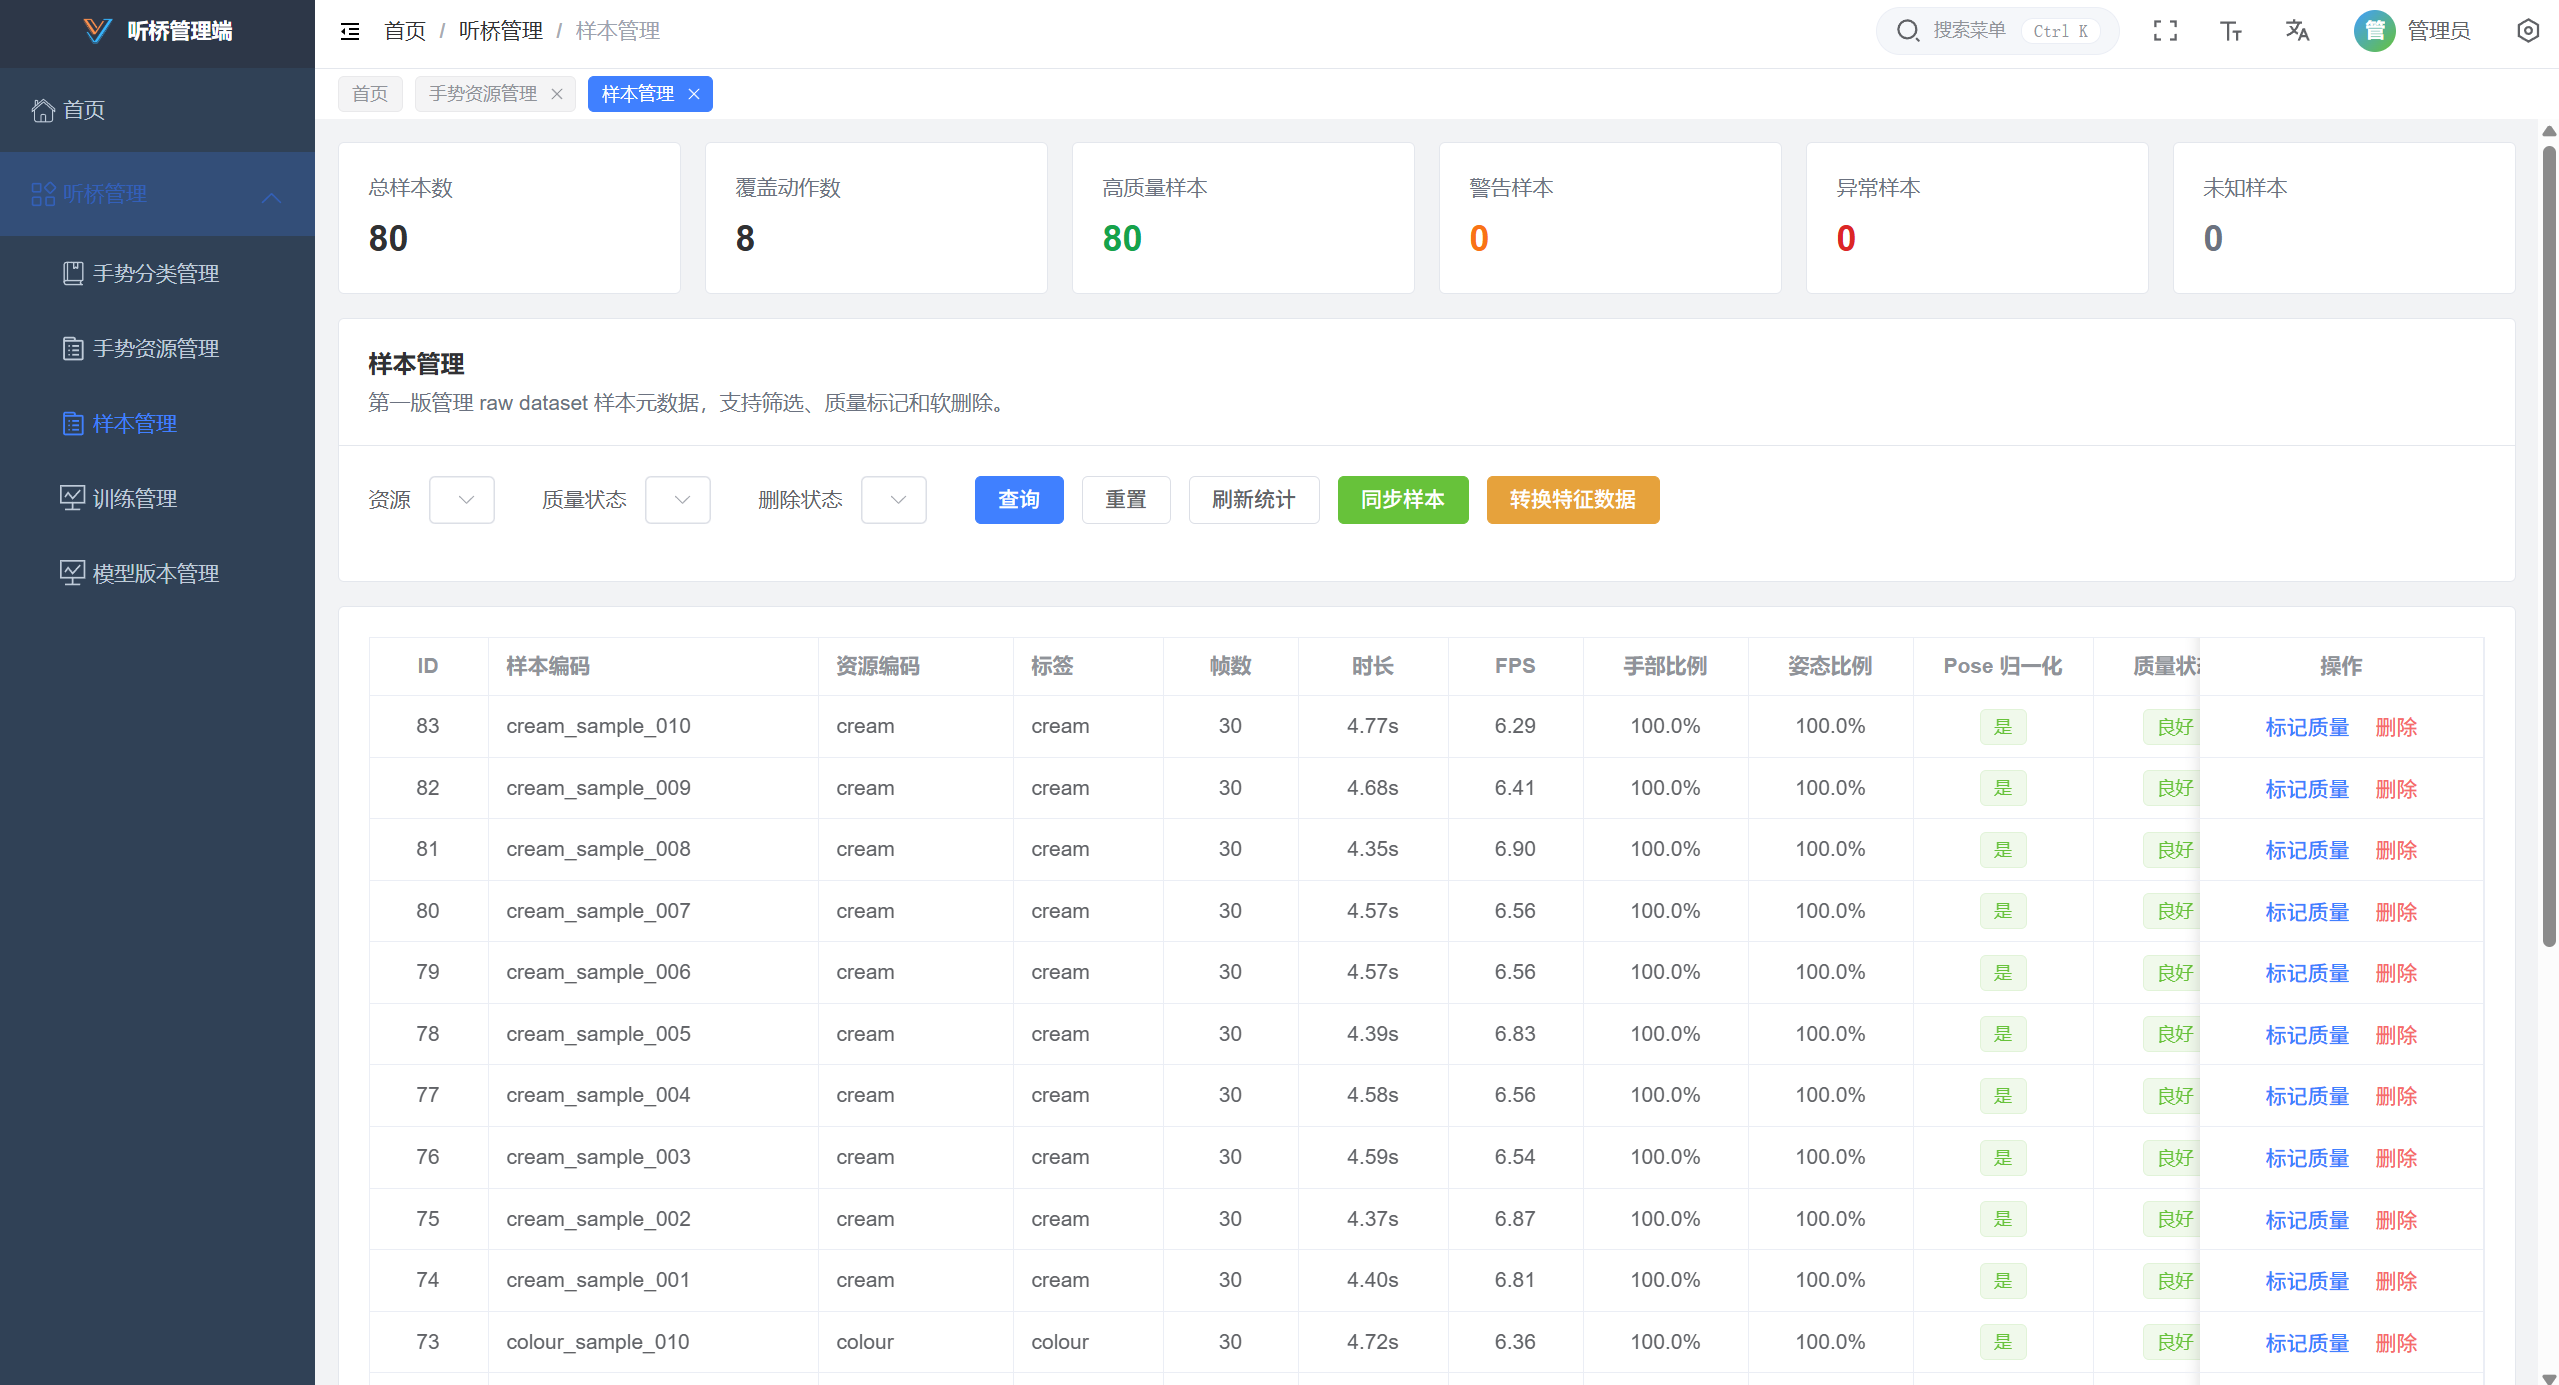
\includegraphics[width=\textwidth,height=0.23\textheight,keepaspectratio]{figures/chapter05/sample-management.png}
    \caption{样本管理}
  \end{subfigure}
  \hfill
  \begin{subfigure}[t]{0.47\textwidth}
    \centering
    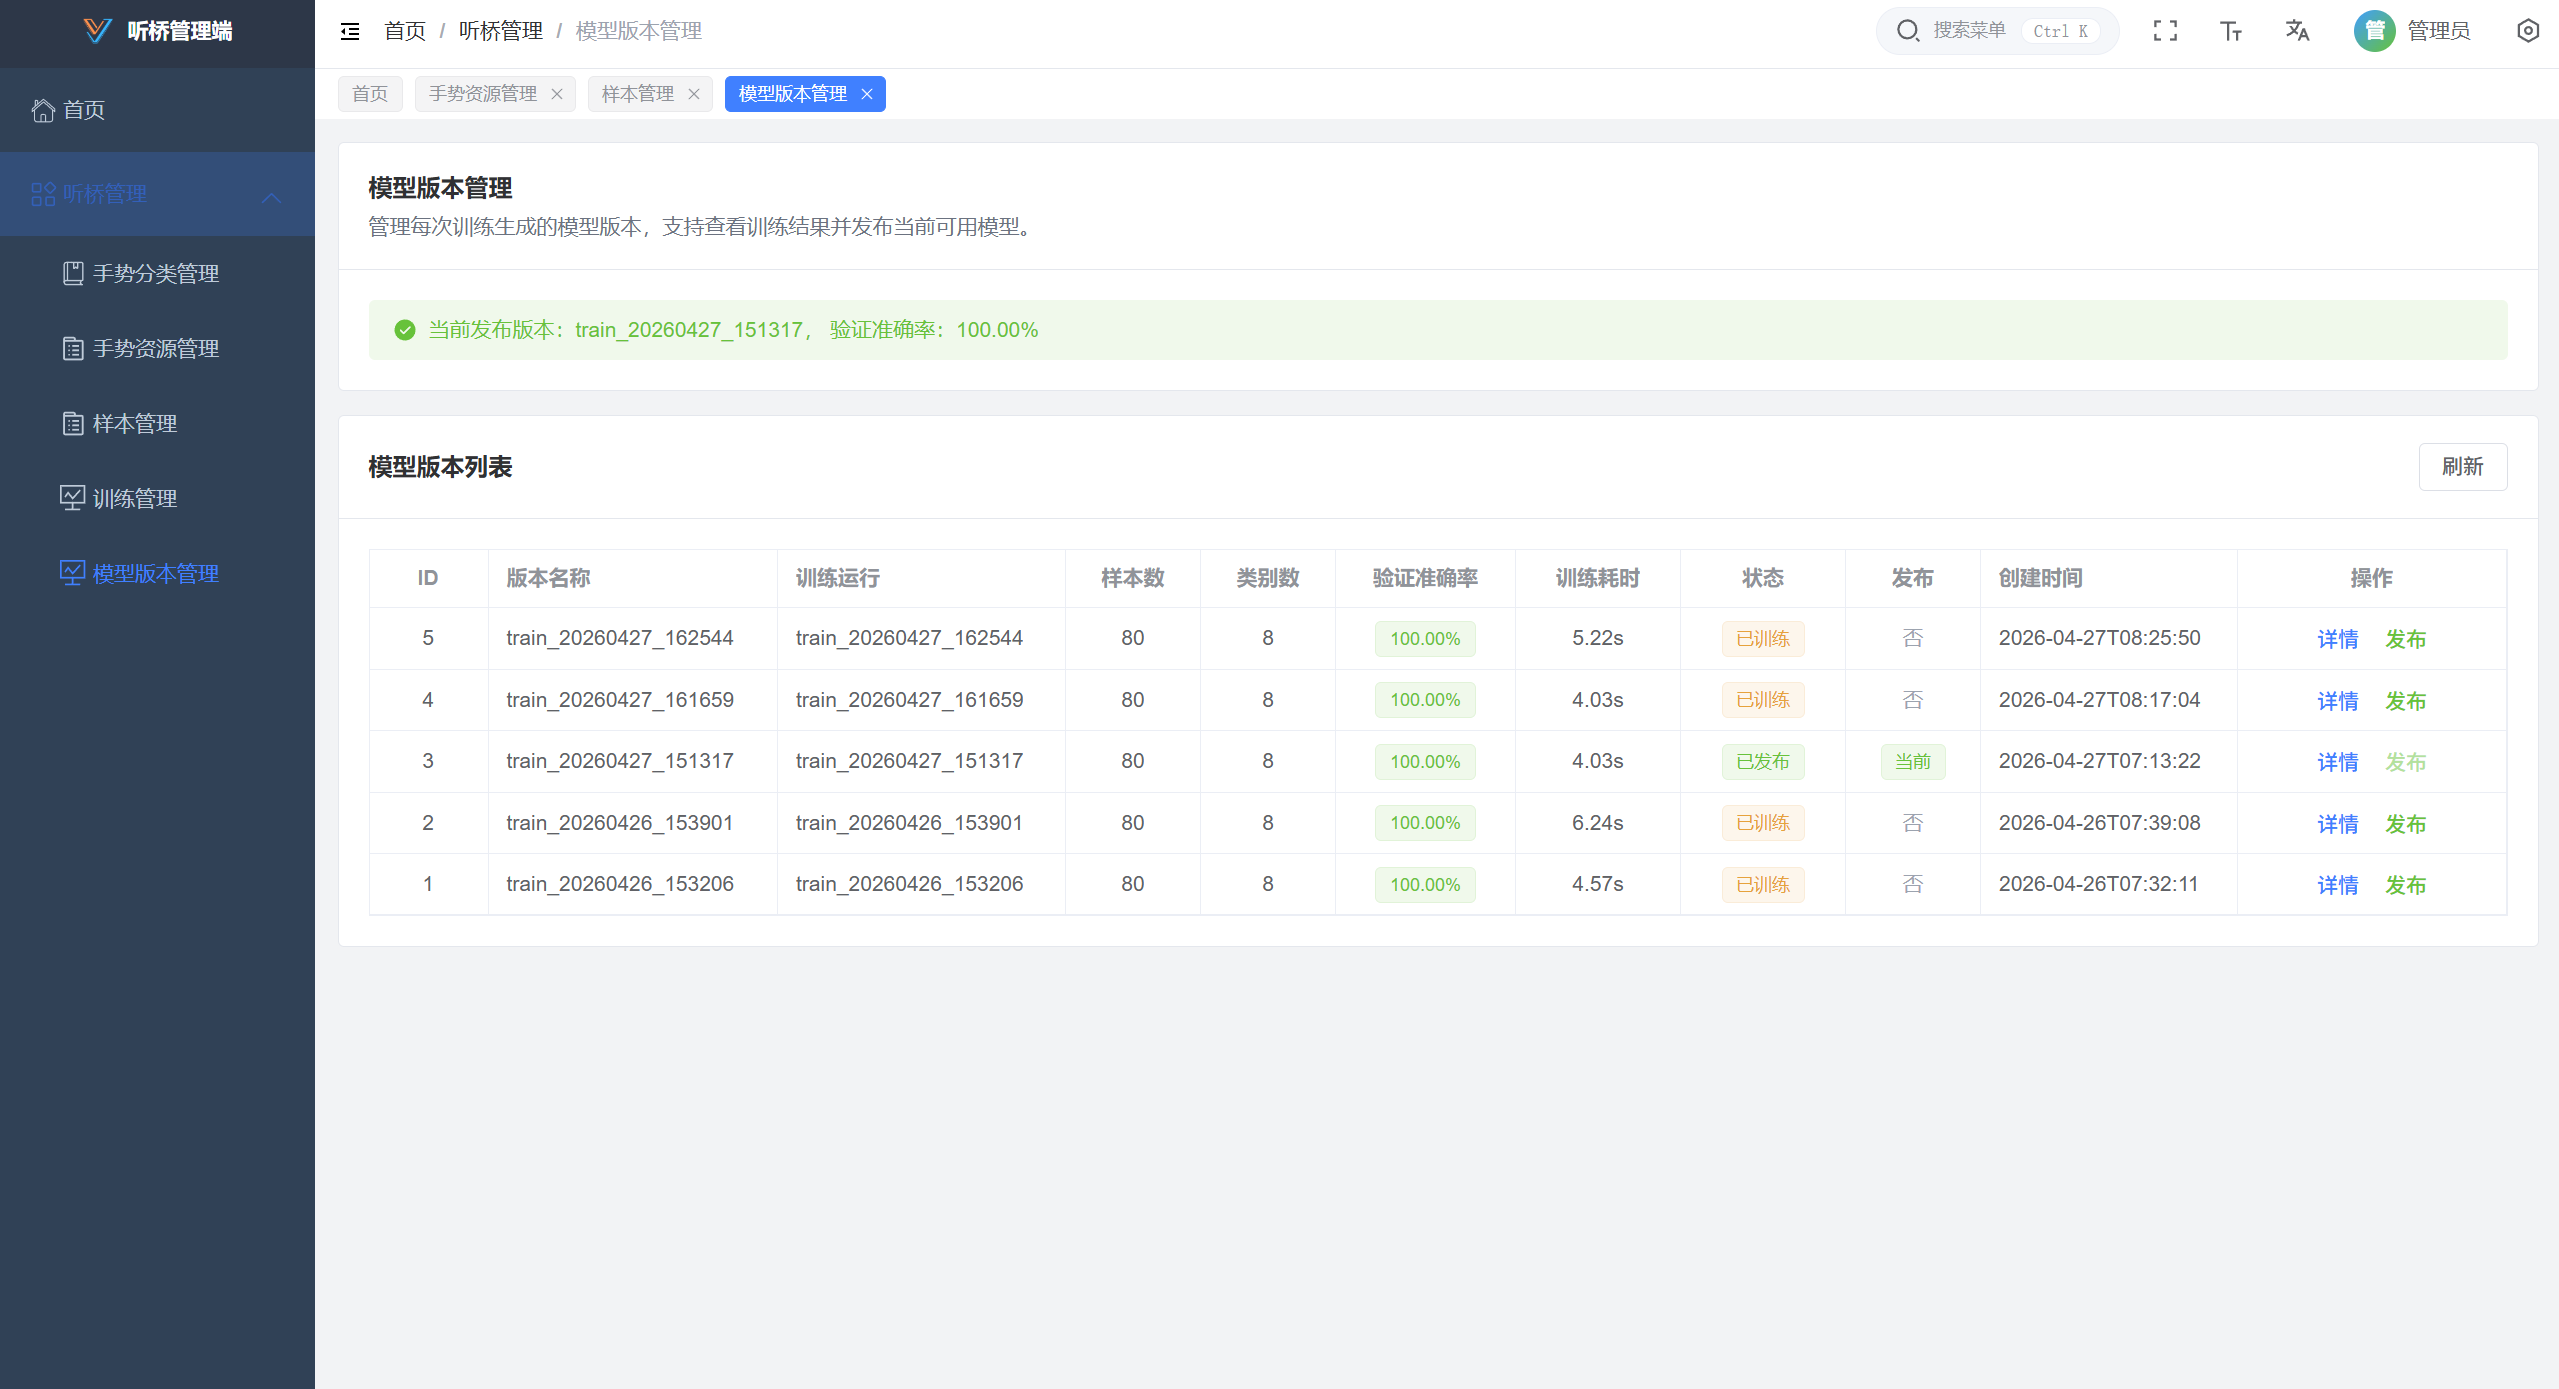
\includegraphics[width=\textwidth,height=0.23\textheight,keepaspectratio]{figures/chapter05/model-version-management.png}
    \caption{模型版本管理}
  \end{subfigure}

  \caption{后台管理端核心页面组织图}
  \label{fig:chapter05-admin-management-pages}
\end{figure}

后台管理端主要功能接口如表~\ref{tab:chapter05-admin-interfaces} 所示。

\WhuInterfaceTable{后台管理端主要功能接口}{tab:chapter05-admin-interfaces}{
登录认证 & POST & /admin/auth/login & 管理员登录并获取 token \\
系统概览 & GET & /admin/dashboard/overview & 获取资源、样本和模型概览数据 \\
分类管理 & GET/POST & /admin/sign/categories & 手势分类分页查询、新增和修改 \\
资源管理 & GET/POST & /admin/sign/resources & 手势资源分页查询、新增和修改 \\
样本管理 & GET/POST & /admin/sign/samples & 样本查询、删除和质量状态维护 \\
训练管理 & POST & /admin/training/start & 触发模型训练任务 \\
模型版本 & POST & /admin/model-versions/publish & 发布当前可用模型版本 \\
}

\subsection{登录认证与路由控制实现}

后台管理端首先实现管理员登录功能。
管理员输入账号和密码后，前端调用服务端登录接口，服务端校验通过后返回 token 和管理员基本信息。
前端将 token 保存到本地，并在后续请求中自动携带该 token。
若服务端返回登录失效或权限异常，前端会清理本地登录状态并跳转回登录页。

后台管理端采用基于路由的页面组织方式。
登录成功后进入后台主布局，主布局通常由侧边栏、顶部栏和内容区域组成。
侧边栏提供系统概览、手势分类管理、手势资源管理、样本管理、训练管理和模型版本管理等入口；
顶部栏用于展示当前管理员信息、退出登录和修改密码等操作；
内容区域根据当前路由展示具体业务页面。

路由守卫用于控制未登录用户访问后台页面。
当用户直接访问管理端内部路由时，前端会先判断本地是否存在有效 token，若不存在则跳转到登录页。
通过这种方式，后台管理端在前端层面实现了基本访问保护，同时服务端仍会在接口层面进行 token 校验，避免仅依赖前端控制。

此外，后台管理端还需要处理 token 过期、退出登录和修改密码等状态变化。
当接口返回登录失效状态时，前端应清除本地 token 和管理员信息，并引导用户重新登录。
通过登录认证和路由控制的结合，后台管理端能够形成较完整的访问控制流程。

\subsection{手势分类与手势资源管理实现}

手势分类管理用于维护移动端资源展示的分类基础。
管理员可以在后台新增、修改、删除或启用禁用分类。
分类信息通常包括分类名称、分类编码、排序值和状态等字段。
前端页面通过表格展示分类列表，并提供新增、编辑和删除等操作入口。
管理员提交表单后，前端调用服务端接口完成数据更新。

手势资源管理是后台管理端的核心功能之一。
管理员可以维护每个手势资源的资源编码、资源名称、所属分类、封面资源、动作示范资源和启用状态等信息。
资源编码与识别服务中的标签体系存在对应关系，因此在资源维护时需要保证资源编码具有稳定性，避免移动端训练资源与模型输出标签之间产生不一致。

在页面实现上，手势资源管理通常采用“查询表格 + 编辑弹窗 + 文件上传”的形式。
表格用于展示资源列表，筛选条件用于按名称、分类或状态查询资源；
编辑弹窗用于填写资源字段；
文件上传组件用于上传封面或动作示范资源。
上传成功后，前端将文件地址与资源表单一起提交给服务端，由服务端保存资源元数据和文件访问路径。

通过分类管理和资源管理，后台管理员可以在不修改移动端代码的情况下扩充或调整训练内容。
移动端通过接口读取已启用的分类和资源，从而动态展示最新训练内容。
这种实现方式使系统内容维护与用户端展示相互解耦，提高了资源管理效率。

\subsection{样本管理与模型训练管理实现}

样本管理用于查看和维护手势识别训练所需的数据。
样本数据通常与具体手势资源关联，后台页面需要展示样本所属标签、样本文件地址、样本质量状态、样本来源和样本状态等信息。
管理员可以查看样本列表，筛选某个手势资源下的样本，也可以删除明显错误或质量较差的样本。

样本管理的意义在于为模型训练提供可控的数据基础。
由于手势识别效果高度依赖训练样本质量，系统需要为管理员提供样本查看和筛选能力。
对于采集到的低质量样本，管理员可以通过后台进行删除或标记，从而减少其对后续模型训练的影响。

模型训练管理用于触发或查看模型训练相关任务。
后台管理端向服务端发送训练请求，由服务端进一步调用 Python 手势识别服务完成特征转换和模型训练。
训练完成后，Python 服务或服务端将训练结果保存为模型文件、标签映射文件和评估指标，再由服务端登记为模型版本。
后台管理端负责展示训练状态和训练结果，使管理员能够了解模型训练是否成功以及模型效果是否满足发布条件。

在当前系统实现中，样本管理、模型训练管理和模型版本管理共同构成识别能力更新闭环。
样本管理提供数据基础，模型训练管理生成模型产物，模型版本管理负责登记和发布模型。
通过该闭环，系统能够在新增样本或扩充动作类别后重新训练模型，并将新模型发布到识别服务中。

\subsection{模型版本管理实现}

模型版本管理用于维护识别模型的版本信息和发布状态。
每个模型版本通常包含版本名称、模型文件地址、标签映射文件地址、支持动作数量、训练样本数量、准确率和发布状态等信息。
管理员可以在后台查看所有模型版本，并选择某个版本进行发布。

在页面实现上，模型版本管理通常以表格形式展示版本名称、支持动作数量、样本数量、准确率、创建时间和发布状态等信息。
管理员可以根据模型版本状态判断当前模型是否可用，也可以通过发布操作将指定模型设置为当前识别服务使用的模型。

模型版本管理需要与样本管理、训练管理和 Python 识别服务保持联动。
训练完成后生成的模型文件和标签映射文件需要登记为模型版本；
管理员发布某一模型版本后，服务端需要更新版本状态，并通知 Python 识别服务加载对应模型。
通过这种方式，后台管理端能够对模型迭代过程进行统一管理。

系统概览页面可以辅助管理员查看资源数量、样本数量、模型版本状态和当前发布模型等信息，但其主要作用是提供全局状态摘要。
模型版本管理本身更关注模型版本数据维护、发布状态控制和识别服务联动，是后台管理端模型维护闭环中的关键模块。

% !TEX root = ../../main.tex

\section{模型版本发布与识别服务联动实现}

模型版本发布与识别服务联动是 HearBridge 系统模型维护闭环中的关键流程。
后台管理端完成模型训练或上传模型文件后，需要在服务端登记模型版本信息，包括版本名称、模型文件地址、标签映射文件地址、支持动作数量、训练样本数量、准确率和发布状态等内容。
服务端通过模型版本表保存这些信息，并向后台管理端提供模型版本查询、发布和状态维护接口。

模型发布的核心目标是保证系统运行时使用明确的当前模型版本。
管理员在后台选择某一模型版本并发布后，服务端需要更新数据库中的发布状态，使同一时刻只有一个模型处于当前发布状态。
随后，服务端调用 Python 识别服务的模型重载接口，使实时识别和视频识别使用最新模型文件。

模型版本发布与识别服务联动流程如图~\ref{fig:model-release-flow} 所示。

\WhuImageFigure[0.78\textwidth][0.52\textheight]{figures/chapter05/model-release-flow.pdf}{模型版本发布与识别服务联动流程图}{fig:model-release-flow}

模型版本发布联动还需要考虑服务状态和错误处理。
如果 Python 识别服务加载模型失败，服务端应向后台管理端返回明确错误，而不能只更新数据库状态。
若模型文件地址、标签映射文件或版本参数不完整，也应在发布前进行校验。
通过这种方式，模型版本管理不仅是后台数据维护功能，也承担识别服务运行状态切换的控制作用。

在移动端实时识别场景中，识别结果中可以返回当前模型版本名称，使用户和开发者能够判断识别结果来自哪个模型版本。
该信息对于后续排查识别效果、分析模型更新前后差异具有一定价值。
通过服务端模型版本管理和 Python 识别服务加载机制的配合，系统形成了从样本维护、模型训练、版本登记到模型发布的基本闭环。

% !TEX root = ../../main.tex

\section{系统异常处理与用户反馈实现}

HearBridge 系统由移动端、后台管理端、Spring Boot 服务端和 Python 手势识别服务协同组成，功能链路中涉及接口调用、文件上传、实时通信、模型加载和语义修正等多个环节。
因此，系统需要对常见异常进行统一处理，并将底层错误转换为用户能够理解的提示信息。

在移动端场景中，常见异常包括登录状态失效、网络连接失败、相机权限不可用、WebSocket 连接中断、未检测到有效动作、视频文件选择失败和视频识别失败等。
对于这些情况，移动端应通过页面提示、加载状态、错误弹窗或结果区域提示等方式向用户说明当前状态，避免用户停留在无反馈界面。

在后台管理端场景中，常见异常包括管理员登录失效、资源字段缺失、资源编码重复、文件上传失败、样本删除失败、训练任务触发失败和模型发布失败等。
对于新增、修改、删除和发布等关键操作，后台管理端应提供必要的确认提示，并在操作完成后展示成功或失败反馈。
对于模型发布这类会影响识别服务运行状态的操作，系统应特别注意数据库状态与识别服务实际加载状态的一致性。

在服务端实现中，异常处理需要覆盖参数校验、权限校验、数据库访问、对象存储访问、外部服务调用和识别服务调用等情况。
服务端不应直接将底层异常暴露给前端，而应转换为统一响应结构，包含状态码、错误信息和必要的业务说明。
这样可以降低前端处理复杂度，也可以避免用户看到难以理解的系统错误。

在句子视频识别链路中，可能出现视频文件上传失败、视频格式不支持、Python 识别服务不可用、模型未加载、语义修正服务调用失败等问题。
服务端需要将这些错误转换为移动端可理解的提示信息。
若语义修正失败但基础识别成功，系统仍可以返回原始识别结果和中文映射结果，并提示语义修正暂不可用。
这样可以避免单个外部服务异常导致整个识别流程完全不可用。

通过异常处理和用户反馈机制，系统能够在复杂链路下保持较好的可用性和可理解性。
用户侧可以明确知道当前操作是否成功、失败原因是什么以及是否可以重新尝试；
管理员侧可以根据提示判断资源维护、样本处理或模型发布是否完成。
该机制有助于提升系统整体稳定性和使用体验。

% !TEX root = ../../main.tex

\section{本章小结}

本章围绕 HearBridge 系统核心功能实现展开说明。
首先，介绍了 HarmonyOS 移动端的启动登录、资源浏览、实时训练交互和句子视频识别页面实现；
其次，说明了 Spring Boot 服务端的分层结构、认证登录态维护、资源服务、句子视频识别服务、DeepSeek 语义修正服务、文件上传与资源访问以及关键接口调用；
随后，介绍了 Vue 后台管理端在登录认证与路由控制、分类资源管理、样本与模型训练管理以及模型版本管理方面的实现；
接着，说明了模型版本发布与 Python 识别服务重载之间的联动过程；
最后，分析了系统异常处理与用户反馈机制。

通过本章实现说明，可以看出 HearBridge 系统并非由单一端完成全部功能，而是通过移动端、后台管理端、Spring Boot 服务端和 Python 识别服务的协同实现核心业务闭环。
下一章将在系统实现的基础上，对手势识别服务实现过程和识别实验结果进行进一步分析。

